%
% Qualificacao_Doutorado.tex (LateX)
% 
% Objetivo: Arquivo principal do relatório de qualificação de doutorado.
% baseado em um template para a geração de documentos em LaTeX.
% 
% Versão 1.0
% 
% Site: http://www.dirackslounge.online
% 
% Programador: 
%		(1.4) - Lauro César Araujo 
%			Template, distribuição e manutenção
%		(1.5) - Rodolfo A. C. Neves (Dirack) 07/10/2019 
%			Modificações e utilização neste relatório
% 
% Email: rodolfo_profissional@hotmail.com
% 
% Licença (Versão modificada): GPL-3.0 <https://www.gnu.org/licenses/gpl-3.0.txt>.
%
% Licença (Versão original): LaTeX Project Public License (LPPL - 1.3) <http://www.latex-project.org/lppl.txt>
%
% Documentação extra: <http://abntex2.googlecode.com/>

\documentclass[
	% -- opções da classe memoir --
	12pt,				% tamanho da fonte
	openright,			% capítulos começam em pág ímpar (insere página vazia caso preciso)
	oneside,			% para impressão em verso e anverso. Oposto a oneside
	a4paper,			% tamanho do papel. 
	% -- opções da classe abntex2 --
	%chapter=TITLE,		% títulos de capítulos convertidos em letras maiúsculas
	%section=TITLE,		% títulos de seções convertidos em letras maiúsculas
	%subsection=TITLE,	% títulos de subseções convertidos em letras maiúsculas
	%subsubsection=TITLE,% títulos de subsubseções convertidos em letras maiúsculas
	% -- opções do pacote babel --
	english,			% idioma adicional para hifenização
%	french,				% idioma adicional para hifenização
%	spanish,			% idioma adicional para hifenização
	brazil				% o último idioma é o principal do documento
	]{abntex2}

\usepackage{multirow}
\usepackage{amsmath}
\usepackage{tocloft}
\usepackage{cmap}			% Mapear caracteres especiais no PDF
\usepackage{lmodern}			% Usa a fonte Latin Modern			
\usepackage[T1]{fontenc}		% Seleção de códigos de fonte.
\usepackage[utf8]{inputenc}		% Determina a codificação utiizada (conversão automática dos acentos)
\usepackage{makeidx}            	% Cria o indice
\usepackage{amssymb,amsfonts,amsmath,wasysym}
\usepackage{lastpage}			% Usado pela Ficha catalográfica
\usepackage{indentfirst}		% Indenta o primeiro parágrafo de cada seção.
\usepackage{nomencl} 			% Lista de simbolos
\usepackage{color}			% Controle das cores
\usepackage{graphicx}			% Inclusão de gráficos
\usepackage{microtype} 			% para melhorias de justificação
\usepackage{subfig}
\usepackage{float} 			% Colocar a figura no local certo
\usepackage{scalefnt} 			% Pacote da redimensionar a fonte de tabelas, figuras e equações.
\usepackage{placeins}
\allowdisplaybreaks
\usepackage{kantlipsum}
\usepackage{pdfpages}
\usepackage{titlesec}
\usepackage[brazilian,hyperpageref]{backref}	 % Paginas com as citações na bibl
\usepackage[alf]{abntex2cite}			 % Citações padrão ABNT
\usepackage{tensor}
\usepackage{setspace}
\usepackage{caption}
\usepackage{amsmath}
\usepackage{enumerate}
\usepackage[portuguese,ruled,lined]{algorithm2e}
\usepackage{algorithmic}

\renewcommand{\figurename}{Figura-}
\usepackage[figurename=Figura]{caption}

\renewcommand{\chapnumfont}{\bfseries}
\renewcommand{\ABNTEXfontereduzida}{\mdseries\footnotesize}
\renewcommand{\ABNTEXchapterfontsize}{\bfseries \normalsize}
\renewcommand{\ABNTEXsectionfontsize}{\normalsize}
\addto{\captionsbrazil}{\renewcommand{\contentsname}{\textbf{SUMÁRIO}}}
\addto{\captionsbrazil}{\renewcommand{\bibname}{\bfseries \textbf{REFERÊNCIAS}\selectfont}}
\renewcommand{\apendicesname}{\bfseries \selectfont  APÊNDICES}
\renewcommand{\apendicename}{\bfseries\selectfont APÊNDICE}
\renewcommand{\anexosname}{\bfseries ANEXOS}

\renewcommand*{\backrefalt}[4]{
	\ifcase #1
	
	\or
	
	\else

	\fi}

%% Informações básicas da CAPA
\instituicao{
  Universidade Federal do Pará -- UFPA
  \par
  Instituto de Geociências
  \par
  Programa de Pós-Graduação em Geofísica}
\titulo{INVERSÃO DO MODELO DE VELOCIDADES NO DOMÍNIO ERC UTILIZANDO AS APROXIMAÇÕES DE TEMPO DE TRÂNSITO SRC NÃO HIPERBÓLICO}

\autor{Rodolfo André Cardoso Neves}
\local{Belém-Pará}
\data{2019}

\orientador{Prof. Dr. João Carlos Ribeiro Cruz}
\coorientador{}

\preambulo{Relatório apresentado ao Programa de Pós-Graduação em Geofísica do Instituto de Geociências 
da Universidade Federal
do Pará, em cumprimento às exigências para obtenção do grau de Doutor em Geofísica.}

\definecolor{blue}{RGB}{41,5,195}
\definecolor{black2}{RGB}{39,64,139}

%% Configurações padrão do PDF
\hypersetup{
		backref=true,
		pagebackref=true,
		bookmarks=true,         		% show bookmarks bar?
		pdftitle={\imprimirtitulo}, 
		pdfauthor={\imprimirautor},
    	pdfsubject={\imprimirpreambulo},
		pdfkeywords={PALAVRAS}{CHAVES}{abnt}{abntex}{abntex2},
	    pdfproducer={LaTeX with abnTeX2}, 		% producer of the document
	    pdfcreator={\imprimirautor},
    	colorlinks=true,       				% false: boxed links; true: colored links
    	linkcolor=black,          			% color of internal links
    	citecolor=black,        			% color of links to bibliography
    	linkcolor=black,          			% color of internal links
    	citecolor=black,        			% color of links to bibliography
    	filecolor=black,      				% color of file links
		urlcolor=black,
		bookmarksdepth=4
}

% Indentação do parágrafo
\setlength{\parindent}{1.3cm}

% Espaçamento entre parágrafos
\setlength{\parskip}{0.2cm}

% Espaçamento entre linhas
\OnehalfSpacing	

% compilar indice
\makeindex

% Compilar lista de abreviaturas e siglas
\makenomenclature

\renewcommand{\sin}{\mathrm{sen}}
\newcommand{\disp}{\displaystyle}
\newcommand{\mbf}{\mathbf}

\hyphenation{geo-fí-si-co}
\hyphenation{MCSEM}

\captionsetup{labelsep=period,font=small,justification=justified,labelfont=md,format=plain,labelsep=endash}

\renewcommand{\imprimircapa}{
\begin{capa}
	\begin{figure}[!t]
		\begin{center}
			
\includegraphics[scale=0.3]{images/Logo_UFPA2.pdf}
		\end{center} 
	\end{figure}
			\begin{center}
				{\ABNTEXchapterfont\bfseries{UNIVERSIDADE FEDERAL DO PARÁ \\ INSTITUTO DE GEOCIÊNCIAS \\ PROGRAMA DE PÓS-GRADUAÇÃO EM GEOFÍSICA} }
		\end{center}

\center

\vspace*{1cm}
{\ABNTEXchapterfont\bfseries\large\MakeUppercase{\imprimirautor}}\\
\vspace*{2cm}
{\ABNTEXchapterfont\bfseries\large\imprimirtitulo}\\
\vspace*{2cm}{\ABNTEXchapterfont\bfseries\large{RELATÓRIO DE QUALIFICAÇÃO DE DOUTORADO}}
\vspace*{\fill}\\
{\large\MakeUppercase{\imprimirlocal}}
\par
{\large\imprimirdata}
\vspace*{1cm}
\end{capa}
}


\makeatletter
\renewcommand{\folhaderostocontent}{
\begin{center}
	\vspace*{1cm}
	{\ABNTEXchapterfont\bfseries\large\MakeUppercase{\imprimirautor}}\\
	\vspace*{\fill}\vspace*{\fill}
	{\ABNTEXchapterfont\bfseries\large\imprimirtitulo}\\
	 \vspace{\baselineskip}
	{\ABNTEXchapterfont\bfseries\large{RELATÓRIO DE QUALIFICAÇÃO DE DOUTORADO}}
	\vspace{\baselineskip}
	\vspace{\baselineskip}
	\vspace*{\fill}
	\abntex@ifnotempty{\imprimirpreambulo}{
	\hspace{5cm}
	\begin{minipage}{10cm}
	\SingleSpacing
	\imprimirpreambulo\\ \\
	{\imprimirorientadorRotulo~Prof. Dr. João Carlos Ribeiro Cruz}\\
	\end{minipage}
	\vspace*{\fill}
	}
	\abntex@ifnotempty{\imprimircoorientador}{
	{\large\imprimircoorientadorRotulo~\imprimircoorientador}
	}
	\vspace*{\fill}
	{\large\imprimirlocal}
	\par
	{\large\imprimirdata}
	\vspace*{1cm}
\end{center}

}

\makeatother

\begin{document}

\imprimircapa

\imprimirfolhaderosto*

\begin{dedicatoria}
   \vspace*{\fill}
   \vspace*{13cm}
   \centering
   \noindent
   \begin{flushright} Dedico este trabalho \`a minha fam\'ilia.
   \end{flushright}
     \vspace*{\fill}
\end{dedicatoria}

\begin{agradecimentos}[\fontsize{12pt}{\baselineskip}\textbf{AGRADECIMENTOS}]
\vspace*{1.5cm}

Ao Prof. Dr. João Carlos pela orientação desta tese, e pela proposta do tema. Além
do suporte e paciência em responder as minhas dúvidas, e das sugestões inteligentes na solução de problemas
que foram aparecendo no caminho.

Agradeço ao professor Sergey Fomel, que apesar de não conhecer pessoalmente, produziu trabalhos
que inspiraram o tema, e disponibilizou gratuitamente
vários
dos programas aqui utilizados.

Agradeço à minha mãe Regina de Nazaré,
à minha irmã Rebeca Cristina, às minhas sobrinhas Ágatha e Anadora, 
e ao meu pai Ricardo Neves, por todo apoio e dedicação
durante a árdua caminhada para a realização deste sonho!

E agradeço à amizade de amigos que conquistei durante o curso de Geofísica, e que de forma direta ou indireta
me ajudaram na realização do trabalho:
Leonardo Reis, Hugo Souza, Diogo Rezende, Antônio Rizimar e Raphael Di Carlo.

\end{agradecimentos}

\begin{epigrafe}
    \vspace*{\fill}
	\begin{flushright}
		\textit{``Todas as coisas excelentes são tão difíceis quanto raras''. \\
		(Baruch Spinoza)}
	\end{flushright}
\end{epigrafe}

\begin{resumo}[\fontsize{12pt}{\baselineskip}\textbf{RESUMO}]
\OnehalfSpacing
O método do elemento de reflexão comum (ERC) é uma alternativa para os métodos
usuais de empilhamento ou migração para a seção de afastamento nulo. Porém, diferente do empilhamento 
convencional, em que os pares são dispostos em famílias de ponto médio comum (PMC) de maneira simétrica ao 
PMC central, a disposição dos pares fonte-receptor é assimétricamente disposta em famílias ERC. 
Haverá pontos sobre a curva ERC onde não existem dados adiquiridos e será necessário realizar a interpolação. 
Assim, o empilhamento ERC pode ser realizado, mesmo a partir de uma 
aquisição sísmica convencional e de dados organizados em famílias PMC.
 \vspace{\onelineskip} 
 \noindent
 \par Palavras-chave: Empilhamento Superfície de Reflexão Comum (SRC). Aproximações não hiperbólicas do tempo de trânsito SRC. 
 Interpolação Elemento de Reflexão Comum (ERC). 
\end{resumo}

\begin{resumo}[\fontsize{12pt}{\baselineskip}\textbf{ABSTRACT}]
\OnehalfSpacing
The common reflection element method (CRE) is an alternative to usual stacking and migration methods 
in zero offset section domain. Besides convencional stacking, wich source receiver pairs are simetricaly distributed into common 
midpoint gathers (CMP) in the neighboorhood of a central CMP, in CRE gathers the disposition of 
source-receiver pairs is assimetric. There are points in CRE curve where there is no data and interpolation is crucial. 
So, CRE gather interpolation can be used to provide information data 
and allow CRE stacking, despite convencional CMP gather as input.
\vspace{\onelineskip} 
\noindent 
\par Keywords: Padé approximants. Common Reflection Surface (CRS) stacking. Non Hyperbolic CRS.
Common Reflection Element (CRE) interpolation.
\end{resumo}

\renewcommand{\listfigurename}{\fontsize{12pt}{\baselineskip}\textbf{LISTA DE ILUSTRAÇÕES}}
\pdfbookmark[0]{\listfigurename}{lof}
\listoffigures*

\cleardoublepage

\tableofcontents*

\cleardoublepage
 
\mainmatter

%% Inclusão dos capítulos ao documento principal
\chapter{INTRODUÇÃO}
\label{cap1}

A equação do sobretempo normal \cite{dix} é uma aproximação de tempo de trânsito de reflexão válida para pequenos afastamentos
entre os pares fonte receptor na superfície de registro em uma aquisição sísmica. Esta equação foi desenvolvida para modelos de
multicamadas planas horizontais. 
A equação de sobretempo normal é uma aproximação em série de Taylor de segunda ordem para o tempo de trânsito, por isto é
também chamada de aproximação hiperbólica. Todavia, esta aproximação diverge do tempo de trânsito analítico
em grandes afastamentos.

Aproximações de tempo de trânsito não hiperbólicas foram desenvolvidas na literatura,
com o intuito de estender a região de convergência das
aproximações de tempo de trânsito no domínio do afastamento: Estas aproximações utilizam mais de dois termos para aumentar a 
acurácia da análise de velocidades e da correção de sobretempo normal. Cada uma destas aproximações terá
as suas limitações na estimativa das velocidades e na relação afastamento profundidade.

O empilhamento convencional, utilizando as aproximações de sobretempo normal hiperbólicas ou não hiperbólicas, é estendido
para o domínio do Ponto Médio Comun (PMC) a partir do empilhamento Superfície de Reflexão Comum (SRC) de
afastamento nulo: 
O empilhamento é realizado sobre uma superfície de tempo de
trânsito no domínio do meio afastamento $h$ e na vizinhança de um PMC central $m_0$, a partir de
três parâmetros ($R_N$, $R_{NIP}$ e $\beta_0$) dados para cada $m_0$. Este empilhamento SRC é dito de afastamento nulo,
pois o PMC central $m_0$ é escolhido da seção de afastamento nulo $h=0$.
O empilhamento SRC de afastamento nulo possui uma aproximação de tempo de trânsito hiperbólica \cite{jager},
e várias aproximações
de tempo de trânsito SRC foram propostas com o objetivo de estender a região de convergência desta aproximação:
As aproximações do SRC não hiperbólico \cite{fomel1}, as aproximações do SRC quarta ordem
\cite{germam}.

Um caso especial do método de empilhamento SRC, é o empilhamento por Elemento de Reflexão Comum (ERC):
O empilhamento ERC é também realizado no domínio do afastamento $h$ e na vizinhança de um PMC central $m_0$, assim como o
empilhamento SRC. Porém, o empilhamento ERC é feito sobre uma curva de tempo de trânsito de reflexão correspondente ao
conjunto de trajetórias de reflexão que possuem em comun
o mesmo ponto de incidência sobre o refletor.
Este método possui a vantagem de prover
parâmetros importantes para a construção do modelo de velocidades, e utiliza dois dos parâmetros
do método SRC de afastamento nulo ($R_{NIP}$ e $\beta_0$).
A principal desvantagem do método ERC é a interpolação: O empilhamento ERC necessita de 
traços em coordenadas de PMC $m$ e meio afastamento $h$ não coincidentes com as coordenadas
e amostragem dos dados adquiridos.
O objetivo desta pesquisa é propor uma metodologia de inversão do modelo de velocidades utilizando o método ERC para
a obtenção da seção empilhada e de interpolação dos dados observados para possibilitar a amostragem das famílias ERC. 

Propomos a seguinte estratégia de interpolação para a obtenção da seção empilhada ERC:
O algoritmo Very Fast Simulated Aneeling (VFSA) é utilizado para obter os parâmetros do SRC de afastamentos nulo
$R_{NIP}$ e $\beta_0$. Como a obtenção de tais parâmetros é um subproduto do empilhamento SRC esta etapa é comum
aos dois métodos, possibilitanto que os dois sejam realizados em fluxos de trabalho independentes que compartilham os 
mesmos parâmetros, não sendo necessário nenhum procedimento além do usual para o empilhamento SRC convencional.
A trajetória ERC é traçada no plano $m, h$ para estabelecer as coordenadas dos traços pertencentes à família ERC
com uma equação que descreve a trajetória e o a equação de tempo de trânsito ERC \cite{cre}.
Interpolaremos os dados adiquiridos utilizando os filtros adaptativos de predição de erro (FPE) no domínio PMC \cite{liu11}.
Esta etapa possibilita a amostragem adequada para a obtenção das famílias ERC,
uma para cada PMC central $m_0$. 
Finalizadas estas etapas,
obteremos a seção empilhada ERC a partir do empilhamento das amostras sobre uma curva de tempo de trânsito ERC 
pertencentes as famílias ERC. Esta curva é determinada para cadar par $m_0, t_0$ da seção empilhada \cite{cre}.

A principal vantagem do método ERC é não precisar de informação a priori do macromodelo de velocidades. 
Este método poder ser utilizado na obtenção do modelo de velocidades através de alguma etapa de inversão,
como a tomografia \cite{cre}. Para a obtenção do modelo de velocidades propomos a seguinte estratégia:
Utilização de um algoritmo iterativo iniciando com um modelo de velocidades inicial que é atualizado
a cada iteração com o algoritmo VFSA. 
O critério de convergência do modelo de velocidades será a coerência entre
os dados modelados a partir do modelo de velocidades da iteração atual com os dados pré empilhados \cite{mesquita}.

O modelo de velocidades de cada iteração do algoritmo de inversão será produzido a partir de respostas simuladas
de difrações em pontos $m_0, t_0$ escolhidos da seção empilhada ERC com uma equação de tempo de trânsito de difrações
e o espalhamento da amplitude do ponto escolhido $A(m_0, t_0)$ sobre a trajetória de tempo de trânsito, formando
a hipérbole de difração \cite{diffractions}. A focalização das difrações na seção empilhada ERC será realizada
através de um algoritmo baseado na continuação de velocidades e na medida de variação máxima local para produzir
os painéis de focalização da imagem com as velocidades que melhor focalizam as respostas de difrações simuladas.
Com o \textit{picking} das velocidades nestes painéis (máximos valores de variação máxima local indicam alta focalização)
é formado o modelo de velocidades da iteração atual \cite{sep_dif}.





%
% cre.tex (LateX)
% 
% Objetivo: Capítulo sobre o método CRE do relatório de qualificação de doutorado.
% 
% Versão 1.0
% 
% Site: http://www.dirackslounge.online
% 
% Programador: Rodolfo A. C. Neves (Dirack) 07/10/2019
% 
% Email: rodolfo_profissional@hotmail.com
% 
% Licença: GPL-3.0 <https://www.gnu.org/licenses/gpl-3.0.txt>.

\chapter{EMPILHAMENTO ELEMENTO DE REFLEXÃO COMUM (ERC)}
\label{cap2:cre}

O método empilhamento Elemento de Reflexão Comum (ERC) é uma alternativa para os métodos de empilhamento PMC ou
migração para a seção de afastamento nulo. Não requer conhecimento do modelo geral em subsuperfície, apenas
o conhecimento da velocidade próxima a superfície é necessário a priori.
O método ERC é baseado somente em considerações cinemáticas em 2D e não é
um processo que preserva as amplitudes.
A principal vantagem do método ERC em comparação com o empilhamento PMC convencional
é que este proporciona a seção empilhada e parâmetros importantes para a construção do macromodelo de 
velocidades que pode inclusive variar lateralmente \cite{cre}.

As principais características do método ERC são:
\begin{enumerate}
 \item[(a)] A construção da seção de afastamento nulo a partir de um conjunto de seções de afastamento constante
com apenas uma estimativa da velocidade próxima da superfície.

 \item[(b)] A determinação dos parâmetros $(R_{NIP},\beta_0)$ para as reflexões de afastamento nulo na seção empilhada.
Estes atributos podem ser utilizados com técnicas de inversão para estimar o macromodelo de velocidades.
\end{enumerate}

Os parâmetros $R_{NIP}$ e $\beta_0$ 
são atributos específicos de uma frente de onda hipotética atribuídos a cada evento de reflexão
primária de afastamento nulo: O raio de curvatura $R_{NIP}$ e o ângulo de emergência $\beta_0$. Esta onda hipotética é
a onda NIP \cite{hubral}.

A idéia principal do método ERC é usar a fórmula do tempo de trânsito ERC no modelo auxiliar para
encontrar a frente de onda NIP que melhor se ajusta aos dados, dado um intervalo
de busca para os parâmetros $R_{NIP}$ e $\beta_0$,
Este processo é semelhante a análise sobretempo normal convencional, todavia enquanto esta análise é feita no
domínio PMC, o método ERC é feito no domínio ERC construído durante o processo. Os parâmetros otimizados $R_{NIP}$ e $\beta_0$
são especificados a partir da análise de coerência nos dados \cite{cre}.

As coordenadas das curvas ERC, mesmo sem o conhecimento da curvatura do refletor em subsuperfície, são definidas
a partir dos parâmetros $R_{NIP}$ e $\beta_0$, obtidos através de um processo de otimização, 
para cada PMC central $m_0$ na seção de afastamento nulo. A Equação que descreve a trajetória ERC no plano $m, h$ \cite{cre}:

\begin{equation}
 \label{eq:2.1}
 m= m_0 + \frac{1}{2\alpha} (1-\sqrt{1+4\alpha^2h^2})
\end{equation}

Onde $\alpha$ é um parâmetro de assimetria que desenpenha um papel importante na seleção de pares fonte-receptor para os quais
os correspondentes raios de reflexão incidem no mesmo ponto sobre o refletor \cite{tygel}. E é dado por:

\begin{equation}
\label{eq:2.2}
 \alpha=\frac{\sin{\beta_0}}{R_{NIP}}
\end{equation}

Os traços sísmicos com as coordenadas $m, h$ dadas pela Equação \ref{eq:2.1} formam uma família ERC.
O método ERC também possui uma aproximação de tempo de trânsito de
reflexão \cite{cre}:

\begin{multline}
\label{eq:2.3}
t(m,h)= \left( \tau_0-\frac{2R_{NIP}}{v_0} \right) 
+\frac{R_{NIP}}{v_0}\sqrt{1-2\alpha(m-m_0+h)+\frac{(m-m_0+h)^2}{R_{NIP}^2}} \\
\end{multline}

Onde $t(m,h)$ é o tempo de trânsito de reflexão no domínio ERC para o PMC $m$ e o meio afastamento $h$.
$v_0$ é a velocidade próxima da superfície, $\tau_0$ é o tempo de trânsito de afastamento nulo e 
$R_{NIP}$ e $\alpha$ são os parâmetros otimizados associados a um PMC central $m_0$.

A Equação \ref{eq:2.3} é utilizada para o empilhamento no domínio ERC. As amostras nas famílias ERC 
que estão sobre esta curva de tempo de trânsito são empilhadas e atribuídas ao PMC central $m_0$ na seção empilhada.
Ao realizar este processo para todos os $m_0$'s da malha obtemos a imagem na seção empilhada ERC.

\begin{figure}[H]
\caption{Representação esquemática de um arranjo ERC para um refletor circular de raio $R$ e profundidade
mínima $D$: A família ERC é formada pelos pares $s_i$-$r_i$ (fonte-receptor) que possuem o mesmo ponto de
reflexão em subsuperfície (ponto $NIP$). A família ERC pode ser entendida a partir de uma fonte pontual explosiva
no ponto $NIP$, que ao ser ativada forma uma frente de onda $NIP$ que atinge a superfície em um PMC central 
$m_0$ com raio de curvatura $R_{NIP}$ e ângulo de incidência $\beta_0$.}
\begin{center}
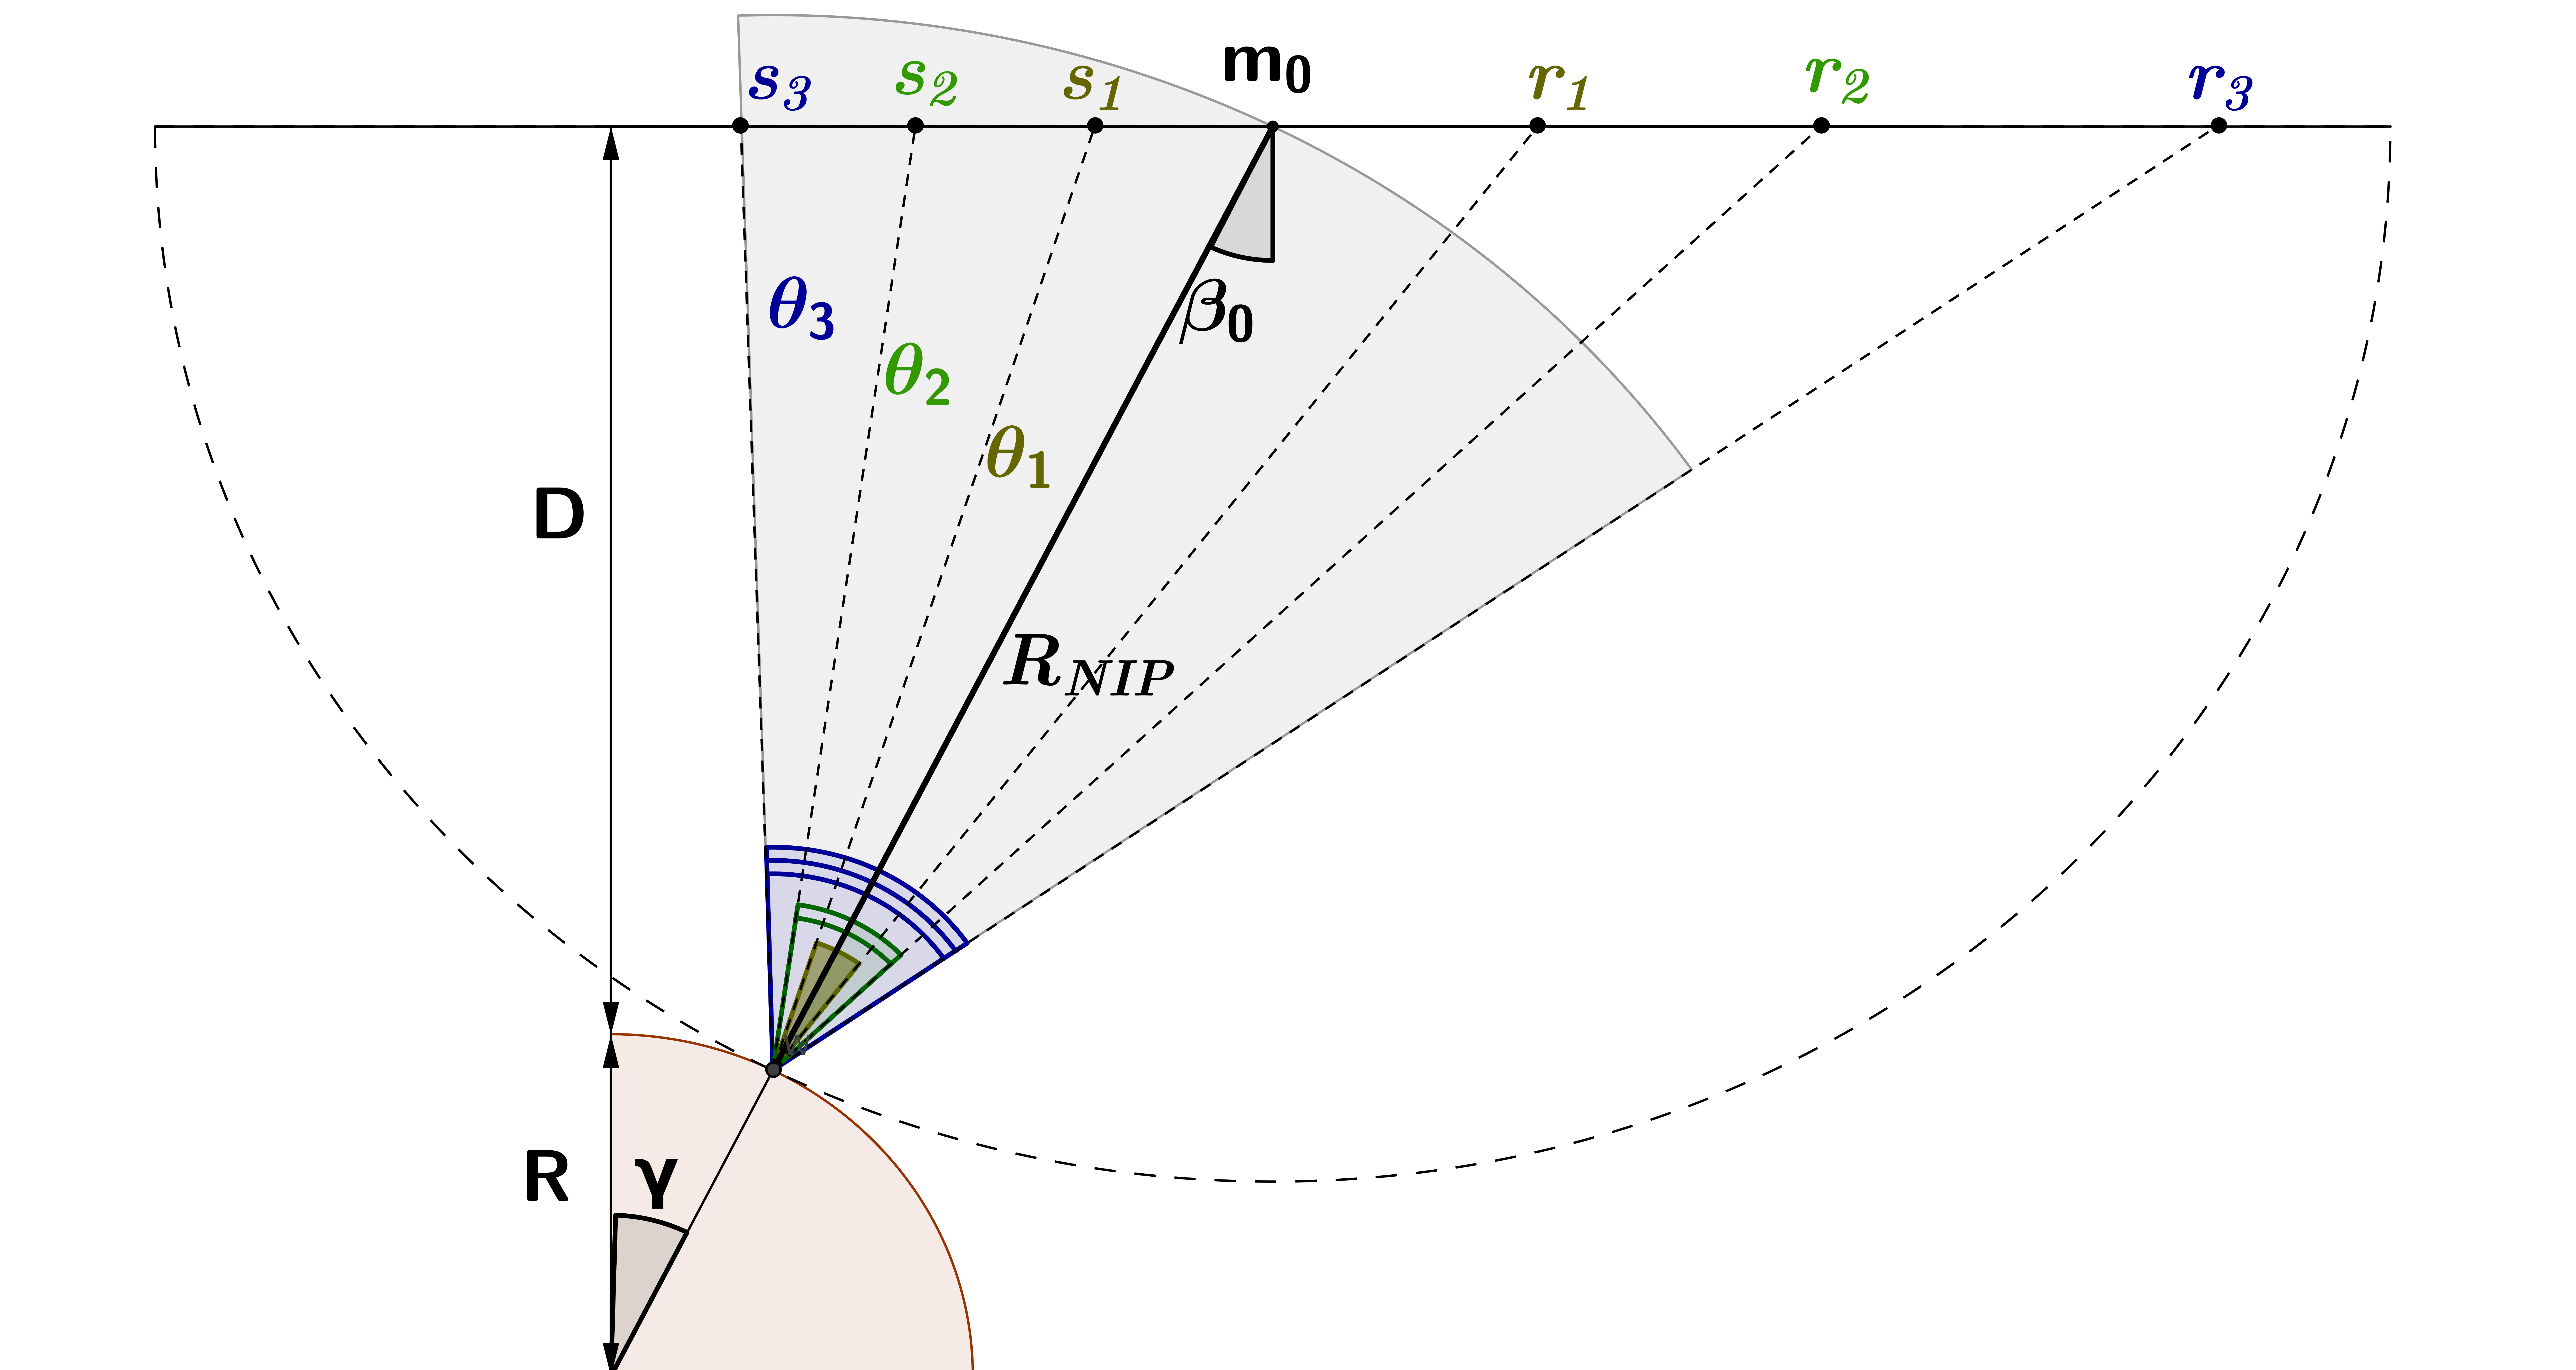
\includegraphics[scale=0.3]{images/cre.png}
\vspace{-0.3cm}
\end{center}
\begin{center}
 Fonte: Do Autor.
\end{center}
\label{fig:2.1}
\end{figure}

O principal desvantagem do método ERC é que as coordenadas de fontes e receptores são distribuídas assimetricamente em tal 
arranjo: Na Figura \ref{fig:2.1} representamos um arranjo ERC em um modelo do refletor circular 
em um meio com velocidade constante $v$.
Todos os raios de reflexão que saem das fontes $s_i$ e chegam aos receptores $r_i$ 
possuem o mesmo ponto de reflexão sobre o refletor.
Porém, a curvatura do refletor estabelece uma distribuição assimétrica dos pares fonte e receptor no domínio do afastamento $h$
e na distância em relação ao PMC central $m_0$, dada por $d=m-m_0$.

A Figura \ref{fig:2.2} mostra as coordenadas $m, h$ de várias curvas ERC hipotéticas com $\alpha$ dado pela Equação \ref{eq:2.2}.
As curvas ERC intersectam as seções de afastamento constante (linhas horizontais na figura) e as seções de ponto médio comum 
(linhas verticais na figura), não sendo posível construir uma malha regular para amostrar tais curvas simultaneamente nos dois
eixos.
A única distribuição que pode ser amostrada regularmente no plano $m, h$ ocorre quando $\alpha=0$. Esta é
a família de ponto médio comum do PMC $m_0$ (linha vertical com pontos em roxo na figura).

A Figura \ref{fig:2.2} mostra as coordenadas $m,h$ de várias curvas ERC hipotéticas com $\alpha$ dado pela Equação \ref{eq:2.2}.
As curvas ERC intersectam as seções de afastamento constante (linhas horizontais) e as seções de ponto médio comum 
(linhas verticais), não sendo posível construir uma malha regular para amostrar tais curvas.
A única distribuição que pode ser amostrada regularmente no plano $m,h$ ocorre quando $\alpha=0$, que corresponderá
a família de ponto médio comum de um dado $m_0$, uma linha vertical no plano (em roxo).

\begin{figure}[htb]
\caption{Representação esquemática das coordenadas de várias trajetórias ERC sobre o plano PMC $m$ x meio afastamento
$h$. As linhas do grid representam as seções de afastamento constante (linhas horizontais) e seções PMC (linhas verticais).
Estas trajetórias foram construídas variando $\beta_0$, $R_{NIP}$ e $\alpha$  na Equação \ref{eq:2.2}. Quando
$\alpha=0$ a trajetória ERC será a trajetória de uma família PMC para um PMC $m_0$.}
\begin{center}
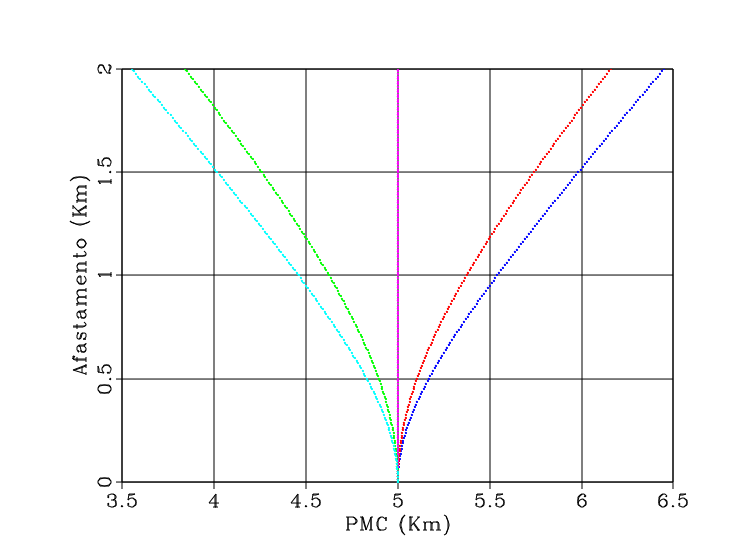
\includegraphics[scale=0.5]{images/creCoord.png}
\vspace{-0.3cm}
\end{center}
\begin{center}
 Fonte: Do Autor.
\end{center}
\label{fig:2.2}
\end{figure}

Neste trabalho propomos uma forma de aumentar a região de convergência da Equação \ref{eq:2.3} utilizando a
aproximação de tempo de trânsito do SRC não hiperbólico e aplicando a condição SDC ($R_N=R_{NIP}$) para
simular a trajetória de tempo de trânsito ERC: No modelo de uma fonte pontual sobre o refletor, o raio de 
curvatura $R_N$ é aproximadamente igual a $R_{NIP}$, esta condição limite é a condição SDC \cite{shav}.

Nossa hipótese é que ao utilizarmos a condição SDC na aproximação de tempo de trânsito do SRC não hiperbólico
teremos uma trajetória de tempo de trânsito ERC com uma região de convergência superior à Equação de tempo de
trânsito ERC (Equação \ref{eq:2.3}).

A aproximação do SRC não hiperbólico possui o
intuito de melhorar a acurácia das aproximações de tempo de trânsito SRC
para grandes afastamentos e separação entre os PMC's \cite{fomel1}.

\begin{equation}
\label{eq:2.4}
 \Phi_{CRS}(h,d;t_0)=\sqrt{\frac{F(d)+ch^2+\sqrt{F(d-h)F(d+h)}}{2}}
\end{equation}

A Equação \ref{eq:2.4} é chamada equação do CRS não-hiperbólico, pois não deriva de uma expansão em série de Taylor
de segunda ordem do tempo de trânsito. Os parâmetros 
$a_1$, $a_2$ e $b_2$
do CRS hiperbólico são utilizados na definição
dos parâmetros do SRC não hiperbólico como \cite{fomel1}:

\begin{equation}
\label{eq:2.5}
 c=2b_2+a_1^2-a_2
\end{equation}

\begin{equation}
\label{eq:2.6}
 F(d-h)=(t_0+a_1(d-h))^2+a_2(d-h)^2
\end{equation}

\begin{equation}
\label{eq:2.7}
 F(d+h)=(t_0+a_1(d+h))^2+a_2(d+h)^2
\end{equation} % Método CRE fundamentos teóricos
\chapter{OTIMIZAÇÃO GLOBAL DOS PARÂMETROS DO SRC DE AFASTAMENTO NULO COM VERY FAST SIMULATED ANEELING}
\label{cap3:vfsa}

O algoritmo Simulated Annealing (SA) é baseado na teoria física da formação de cristais
através do resfriamento lento (Annealing) destes cristais, a partir do seu ponto de fusão \cite{ingber}.
O objetivo do algoritmo é minimizar a função objeto $f(p)$ a patir de perturbações aleatórias do vetor de parâmetros $p$,
para uma nova posição $p'$. O valor $p'$ é avaliado a partir do seguinte critério de aceitação:

\begin{equation}
\label{eq:3.1}
 \Delta f=f(p')-f(p) < 0
\end{equation}

O algoritmo inicia através da escolha de um valor inicial de temperatura, $T=T_0$, para esse valor inicial há
a escolha aleatória do vetor de parâmetros $p_i=(p_1,p_2,p_3,...,p_n)$. O vetor de parâmetros é perturbado 
de sua posição inicial a uma nova posição $p'_i$. Calcula-se o valor da função objeto, $f(p)$ e $f(p')$. Se $f(p')$ é
menor que $f(p)$ significa que o valor da função objeto é menor para o vetor $p'_i$
e a função objeto está convergindo para um mínimo. $p'_i$ é adotado como o
novo vetor de parâmetros, repete-se o processo até atingir o mínimo Global.

Se a Equação \ref{eq:3.1} é satisfeita o valor de $p'$ é aceito como o novo vetor de parâmetros $p$ e o processo
é reiniciado: Perturba-se $p$ para uma nova posição $p'$, e é avaliado se a Equação \ref{eq:3.1} permanece satisfeita. 
Ou seja, a cada nova
iteração a função objeto deverá possuir um valor menor, até que atinja o seu valor mínimo.

Todavia, a função $f(p)$ pode não convergir para o mínimo global, de modo a se manter presa
em um mínimo local. Para tanto, o algoritmo SA permite deslocamentos ascendentes no valor de $f(p)$ a partir de um critério
probabilístico (Critério de Metrópolis): Se $f(p')$ for maior que $f(p)$, a Equação \ref{eq:3.1} não será satisfeita, então
a nova posição $p'$ não será aceita de imediato, devendo passar por um novo teste.

Primeiro, calculamos um número $P$, dado por:

\begin{equation}
\label{eq:3.2}
 P=exp(\frac{-\Delta f}{T})
\end{equation}

E adotamos o seguinte critério probabilístico: 
Se $P$ for maior do que $u$, um número aleatório entre 0 e 1, $p'_i$ será aceito, senão $p'_i$ é
descartado e o algoritmo é reiniciado com uma nova perturbação ao vetor $p$.
Valores baixos de $T$ e altos $\Delta f$ diminuem a probabilidade de que $p'_i$ seja aceito.

O algoritmo Very
Fast Simulated Annealing (VFSA) surgiu com o objetivo de melhorar o desempenho do algoritmo Simulated Annealing (SA). 
Este algoritmo, também é chamado de \textit{Boltzmann Annealing} (BA) e
introduz varias modificações ao
algoritmo padrão SA \cite{ingber}.

No algoritmo VFSA a perturbação de cada elemento $\alpha_{k,i}$ na dimensão $i$ , é realizada
segundo a relação \cite{klaus}:

\begin{equation}
\label{eq:3.3}
 \alpha_{k+1,i}=\alpha_{k,i}+y_i(B_i-A_i)
\end{equation}

Onde $\alpha_{k+1,i}$ é um novo parâmetro obtido a partir do parâmetro $\alpha_{k,i}$ da iteração anterior.
O novo parâmetro é restrito a janela:

\begin{equation}
\label{eq:3.4}
  \alpha_{k+1,i},\alpha_{k,i}\in[A_i,B_i]
\end{equation}

Ou seja, $A_i$ e $B_i$ delimitam o espaço de busca dos parâmetros através da otimização global. 
$u_i$ e $y_i$ são números aleatórios distribuídos da seguinte forma:

\begin{equation}
\label{eq:3.5}
  y_i\in[-1,1]
\end{equation}

\begin{equation}
\label{eq:3.6}
  u_i\in[0,1]
\end{equation}

O cálculo de $y_i$ é dado por:

\begin{equation}
\label{eq:3.7}
  y_i=sgn(u_i-1/2)T_i[(1+1/T_i)^{2u_i-1}-1]
\end{equation}

Onde $sgn()$ é a função sinal, definida da seguinte forma:

%\begin{equation}
$$sgn(t)=1, t > 0$$

$$sgn(t)=-1 t < 0$$
%\end{equation}


O mínimo global pode ser obtido usando a sequência de refriamento $T_i$, definida da seguinte forma \cite{ingber}:

\begin{equation}
\label{eq:3.8}
 T_i(k)=T_{0i}exp(-C_ik^{1/n})
\end{equation}

Onde o parâmetro $T_{0i}$ é a temperatura inicial, e $C_i$ é um parâmetro livre para controle do decaimento e ajuste ao
problema \cite{klaus}. O pseudo-código do algoritmo VFSA é apresentado abaixo \cite{stoffa}:

\vspace{\onelineskip} 

% \begin{algorithm}[H]
% \Entrada{Inicia com um valor aleatório para o parâmetro $m_0$ com uma energia $E(m_0)$}
% \Saida{Parâmetros $p_i$ otimizados}
% \Inicio{
% inicializa\c{c}\~ao\;
% \Repita{fim do texto}{
% leia o atual\;
% \uIf{entendeu}{
% vá para o próximo\;
% próximo se torna o atual\;}
% \Else{volte ao início da seção\;}
% }
% }
% \caption{O pseudo-código do algoritmo Very Fast Simulated Annealing (VFSA).}
% \end{algorithm}


\begin{algorithm}
\label{alg:3.1}
 \Entrada{Inicia com um valor aleatório para o parâmetro $m_0$ com uma energia $E(m_0)$}
\Saida{Parâmetros $m_i$ do modelo otimizados}

\Repita{arrefecer a temperatura $T_0$ em $q$ iterações}{

  Obtenha a temperatura $T_q$ desta iteração para $M$ parâmetros:
  
  $T=T_0*\exp(-C_0*q^{M^-1});$

    \Repita{atualizar todos os parâmetros do modelo $m_i=1,...,M$}{

      Obtenha um número aleatório $u_i \in U[0,1]$\;

      Obtenha a perturbação do parâmetro $y_i=sgn(u_i-\frac{1}{2})T_i'[(1+T_i')^{2u_i-1}-1]$\;

      Perturbe o parâmetro dentro da janela de busca:

      $m_{new}=m_{old}+y_i(m_{max}-m_{min})$\;

      $m_{min}<=m_{new}<=m_{max}$\;}

    Com os novos parâmetros do modelo ($m_{new}$), calcule o delta da função Energia:
    
    $\Delta E=E(m_{new})-E(m_0)$\;
    
    \Se{$E(m_{new})>E(m_0)$}{
    Guarde os parâmetros atuais ($m_{new}$)\;}

    Para atualizar utilize o critério probabilístico de aceitação (critério de Metropolis):
    
    $P=exp(\frac{-\Delta E}{T})$\;

    \Se{ $\Delta E <= 0$}{
      Atualize:
      
      $m_0=m_{new}$\;

      $E(m_0)=E(m_{new})$\;}

    \Se{ $\Delta E > 0$}{
      Escreva um numero aleatório $r=U[0,1]$\;

      \Se{ $P > 0$}{
	Atualize:
	
	$m_0=m_{new}$\;

	$E(m_0)=E(m_{new})$\;}

    }

}
\caption{O pseudo-código do algoritmo Very Fast Simulated Annealing (VFSA).}
\end{algorithm}

\vspace{\onelineskip} 

\begin{figure}[htb]
\caption{Fluxo de processamento do algoritmo de otimização global Very Fast Simulated Aneeling (VFSA)
proposto para obtenção dos parâmetros do SRC de afastamento nulo.}
\begin{center}
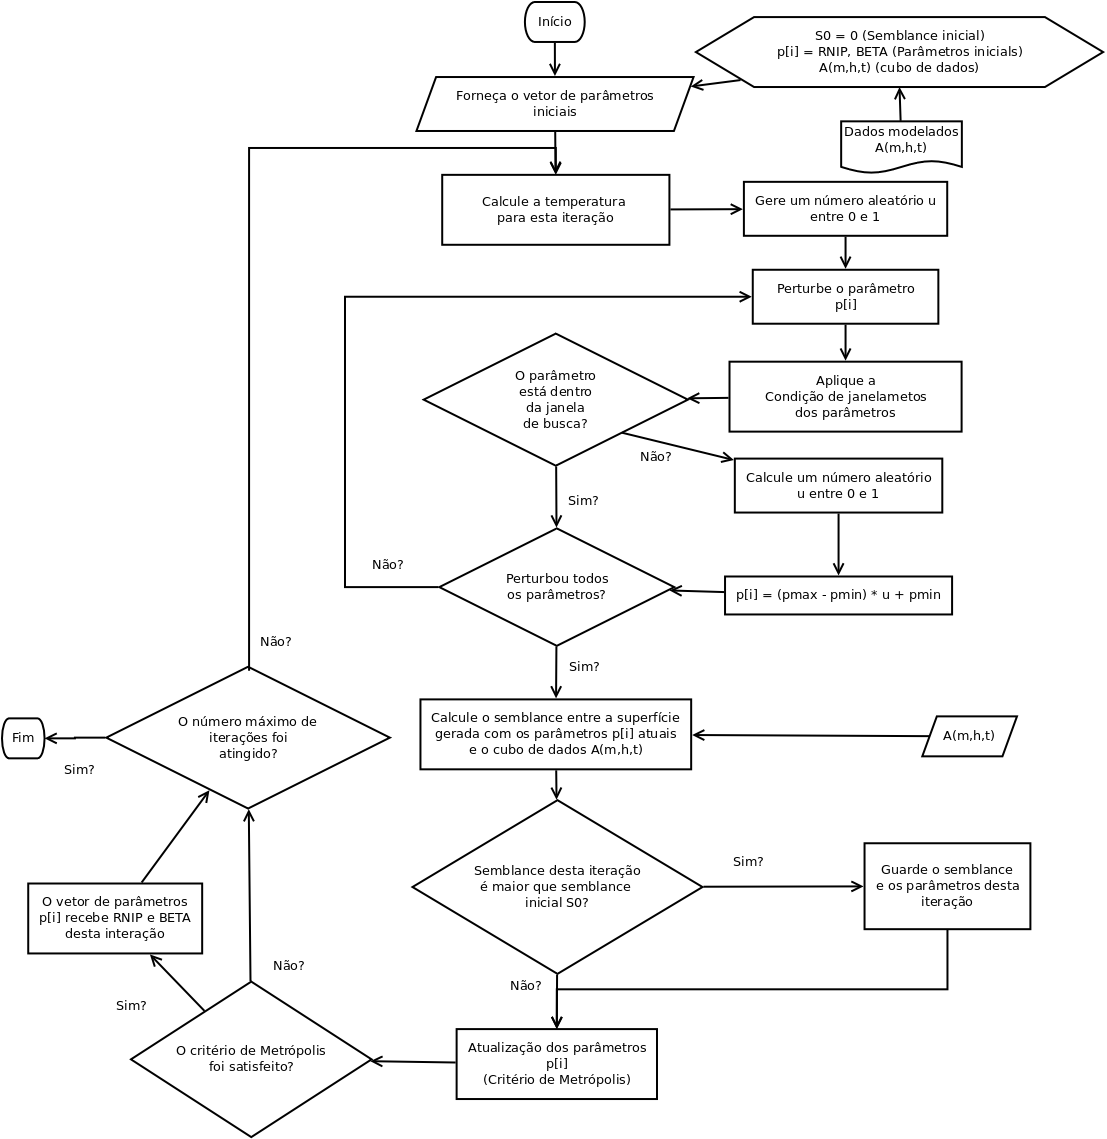
\includegraphics[scale=0.45]{images/VFSA.png}
\vspace{-0.3cm}
\end{center}
\begin{center}
 Fonte: Do Autor.
\end{center}
\label{fig:3.1}
\end{figure}

Podemos utilizar o semblance (coerência) no algoritmo VFSA como critério de convergência na Equação \ref{eq:3.1}
para determinar os parâmetros do SRC $R_N$, $R_{NIP}$ e $\beta_0$. Os dois últimos parâmetros são utilizados também 
no método ERC.

Utilizando uma aproximação de tempo de trânsito SRC, medimos a coerência entre esta aproximação e os
dados no domínio $m, h$, para uma tripla $R_N$, $R_{NIP}$ e $\beta_0$.
A coerência será máxima quando o ajuste entre a aproximação de tempo de trânsito e os dados
for a melhor possível, os parâmetros do SRC que produzirem o melhor ajuste serão o resultado da otimização.

O semblance é uma medida de coerência baseada na soma da energia de traços adjacentes, se os traços alinhados são similares,
a soma dos traços adjacentes será máxima. A definição matemática de semblance para um grupo de $M$ traços, ao 
longo de uma janela de $N$ amostras, na posição $x_j$ e no tempo $t_i$, é dada por \cite{seg}:

\begin{equation}
\label{eq:3.9}
 S_{NM}=\frac{ \sum_{i=1}^N [\sum_{j=1}^M x_j(t_i)]}{M \sum_{i=1}^N \sum_{j=1}^Mx^2_{j}}
\end{equation}

O semblance é a energia da soma dos valores dos traços dividida pela soma da energia dos traços. 
Seu valor máximo é 1 e o mínimo é 0 \cite{seg}. O semblance é medido em uma janela em $m, h$ entre os dados adiquiridos 
e uma superfície de tempo de
trânsito SRC aproximada. 

Para adaptar o Algoritmo \ref{alg:3.1} para o problema da otimização dos parâmetros do SRC, utilizamos a
função Semblance como função Energia $E(m_i)$ e os parâmetros do modelo $m_i$ como o vetor
de parâmetros $m_i={R_N,R_{NIP},\beta_0}$, escolhemos valores arbitrários para constante de amortecimento $C_0$ e
para temperatura inicial $T_0$.

Calculamos o Semblance entre uma superfície de tempo de trânsito SRC, por exemplo a
superfície de tempo de trânsito SRC não hiperbólica (Equação \ref{eq:2.4}) 
e os dados modelados em cada iteração. E utilizamos este valor como critério de
convergência do algoritmo do VFSA na Equação \ref{eq:3.1} 

Isto posto, o problema se torna
uma busca do valor máximo da função energia no decorrer das iterações e por conseguinte dos parâmetros $m_i$ que
produzem tal valor. Os parâmetros $R_N$, $R_{NIP}$ e $\beta_0$ que melhor
ajustam a superfície aproximada aos dados serão os parâmetros ótimos. % Otimização global VFSA
%
% pef.tex (LateX)
% 
% Objetivo: Capítulo sobre o método de interpolação com filtros adaptativos de predição de erro
% (PEF, do inglês) do relatório de qualificação de doutorado.
% 
% Versão 1.0
% 
% Site: http://www.dirackslounge.online
% 
% Programador: Rodolfo A. C. Neves (Dirack) 17/10/2019
% 
% Email: rodolfo_profissional@hotmail.com
% 
% Licença: GPL-3.0 <https://www.gnu.org/licenses/gpl-3.0.txt>.

\chapter{FILTROS ADAPTATIVOS DE PREDIÇÃO DE ERRO (FPE)}
\label{cap4:pef}

Uma restrição comumente utilizada na interpolação de traços sísmicos
é assegurar que os dados interpolados, depois da filtragem,
tenham mínima energia. Isto significa a escolha de valores
nos limites do filtro de modo a minimizar o transiente. Neste ponto os mínimos
quadrados levam grande vantagem, pois tendem a absorver grandes valores e a distribuir
uniformemente os resíduos em tempo e frequência na extensão permitida \cite{claerbout92}.

A filtragem é equivalente a multiplicação espectral. Assim, especificar a filtragem
é o equivalente a preescrever o espectro dos dados interpolados. Uma escolha sensível
é o espectro do dado registrado, que pode ser capturado através dos coeficientes dos
filtros adaptativos de predição de erro (FPE) do dado \cite{spitz}. 

Os FPE, também conhecidos como filtros de autoregressão, desenpenham o
papel da ``matriz inversa de covariância'' da teoria das estimativas na estatística.
O sinal é regredido sobre si mesmo na estimativa dos coeficientes do filtro. O FPE
pode ser implementado no domínio tempo-espaço ou frequência-espaço. Os FPE no tempo-espaço
são menos propensos a criar eventos espúrios na presença de ruído do que os filtros
frequência-espaço \cite{abma}. 

A utilização dos FPE na interpolação ocorre em dois passos:
Primeiro, o FPE é estimado através da minimização da saída da convolução
dos dados conhecidos com o FPE desconhecido. Segundo, os dados interpolados
são estabelecidos a partir da minimização da convolução do FPE anteriormente 
calculado com o modelo conhecido, restringido pelos dados conhecidos \cite{curry}.

Contudo, a busca dos coeficientes do FPE necessita evitar equações regressivas que 
envolvam as fronteiras ou dados ausentes. Isto pode ser feito
criando uma máscara de seleção $K(t,x)$, uma matriz 
diagonal de uns nos traços originais e zeros nos traços a serem interpolados, 
para translações causais e entradas de dados \cite{claerbout10}

Os coeficientes $B_n(t,x)$ do filtro são obtidos
solucionando o problema de mínimos quadrados \cite{liu11}:

\begin{equation}
\label{eq:4.1}
\hat{B_n}(t,x) = \arg \min_{B_n} \left \rVert K(t,x) \left [ S(t,x) - \sum^N_{n=1}B_n(t,x)S_n(t,x) \right ] \right \Arrowvert^2_2 
+ \epsilon^2 \sum^N_{n=1} \left \rVert D [ B_n(t,x) ] \right \Arrowvert^2_2
\end{equation}

Onde $S_n(t,x) = S(t-i,x-j)$, representa a tranlação causal de $S(t,x)$. 
$D$ é um operador de regularização e $\epsilon$ é um parâmetro de regularização escalar.

Se $D$ for definido como um operador linear, a estimativa através dos mínimos quadrados se reduz a uma
inversão linear \cite{liu11, fomel2009}.

\begin{equation}
\label{eq:4.2}
b = A^{-1} d
\end{equation}

Onde:

\begin{equation}
\label{eq:4.3}
 b = \left[ B_1(t,x)\:\: B_2(t,x)\:\: ...\:\: B(t,x) \right]^T
\end{equation}

\begin{equation}
\label{eq:4.4}
 d = \left[ S_1(t,x)S(t,x)\:\: S_2(t,x)S(t,x)\:\: ... \:\: S_N(t,x)S(t,x) \right]^T
\end{equation}

E os elementos da matriz $A$ são:

\begin{equation}
\label{eq:4.5}
 A_{nk}(t,x) = S_n(t,x)S_k(t,x) + \epsilon^2 \delta_{nk}D^TD
\end{equation}

Ao incorporar um operador de suavização $G$ ao invés de $D$ estabelecemos uma janela de suavização
dado o tamanho e a forma do filtro $B_n(t,x)$ e o raio da janela de suavização no espaço e no tempo em $G$ \cite{fomel2007}.
Os coeficientes do filtro nos traços zerados intercalados aos traços originais estão assim restringidos pelos limites
da janela de suavização, dando maior peso aos traços mais próximos.

Isto é feito definindo $G$ como um operador de suavização gaussiano com raio ajustável, obtido através da
aplicação repetida de um filtro triangular e da escolha do parâmetro $\lambda$ como o valor médio de $S_n(t,x)$.
Com estas considerações a inversão toma a forma \cite{liu11, fomel2007}:

\begin{equation}
\label{eq:4.6}
 b = \hat{A}^{-1}\hat{d}
\end{equation}

Onde:

\begin{equation}
\label{eq:4.7}
 \hat{d} = [ G[S_1(t,x)S(t,x)]\:\: G[S_2(t,x)S(t,x)]\:\: ...\:\: G[S_N(t,x)S(t,x)] ]^T
\end{equation}

Os elemetos da matriz $\hat{A}$ são:

\begin{equation}
\label{eq:4.8}
 \hat{A}_{nk}(t,x) = \lambda^2 \delta_{nk} + G[S_n(t,x)S_k(t,x) - \lambda^2 \delta_{nk}]
\end{equation}

A segunda etapa também é resolvida a partir dos mínimos quadrados. Porém,
o filtro já é conhecido e o objetivo agora é estimar os traços desconhecidos.
A partir da seguinte formulação de um novo problema de mínimos quadrados \cite{liu11}:

\begin{equation}
\label{eq:4.9}
 \hat{S}(t,x) = \arg \min_S \left \rVert S(t,x) - \sum^N_{n=1}\hat{B}_n(t,x) S_n(t,x) \right \Arrowvert^2_2
\end{equation}

Sujeito a seguinte restrição dos traços conhecidos:

\begin{equation}
\label{eq:4.10}
 \hat{S}(t,x) = S_{known}(t,x_k)
\end{equation}

Onde $\hat{S}(t,x)$ representa a saída da interpolação.
A minimização é feita a partir do método dos gradientes-conjugados \cite{hestenes}. 
A restrição a partir da Equação \ref{eq:4.3} é utilizada como modelo inicial e restringe
a saída utilizando os traços conhecidos em cada iteração no esquema dos gradientes-conjugados.
O custo computacional é proporcional ao número de iterações multiplicado
pelo tamanho do filtro, o número de amostras no tempo e no espaço $N_i \times N_f \times N_t \times N_x$. 
Crescendo o raio de suavização na regularização decresce o número de iterações no passo da
estimativa do filtro \cite{liu11}.

Os filtros adaptativos de predição de errro (FPE) podem ser utilizados para regularizar os dados sísmicos,
de modo a produzir uma amostragem suficiente para o estabelecimento das seções ERC.
Como representado na Figuras \ref{fig:4.1}, a trajetória ERC calculada para cada $m_0$ não
necessariamente intersecta as seções de afastamento constante nas coordenadas $m_i$, $h_i$ dos traços sísmicos. 
A trajetória ERC calculada passa entre os traços identificados pelas coordenadas $m1,h2$ e $m3, h2$ na Figura \ref{fig:4.1},
sendo necessário aumentar a discretização em $m$ da seção $h2$ para poder amostrar corretamente a trajetória ERC.

Ao intercalar os traços originais com novos traços zerados $m'_i$, e utilizar os filtros adaptativos de predição
de erro para interpolar os valores das amostras em cada traço $m'_i$, dobramos 
a discretização das seções de afastamento constante.
Este processo pode ser repetido até que a discretização seja suficiente para amostrar a curva ERC em cada seção de afastamento
constante (na Figura \ref{fig:4.2}, $m'_2$ está mais próximo da trajetória 
ERC do que $m_3$ e $m_2$ já que a distância 
entre os traços da seção $\Delta m$ é menor).

\begin{figure}
\caption{Representação esquemáticas de uma trajetória ERC para um $m_0$ arbitrário. A trajetória intersecta a seção de
afastamento constante entre dois traços sísmicos identificados pelas coordenadas $m2, h2$ e $m3, h2$, sendo necessário
aumentar a discretização para amostrar corretamente a trajetória. $\Delta m$ é a distância entre os traços da seção.}
\begin{center}
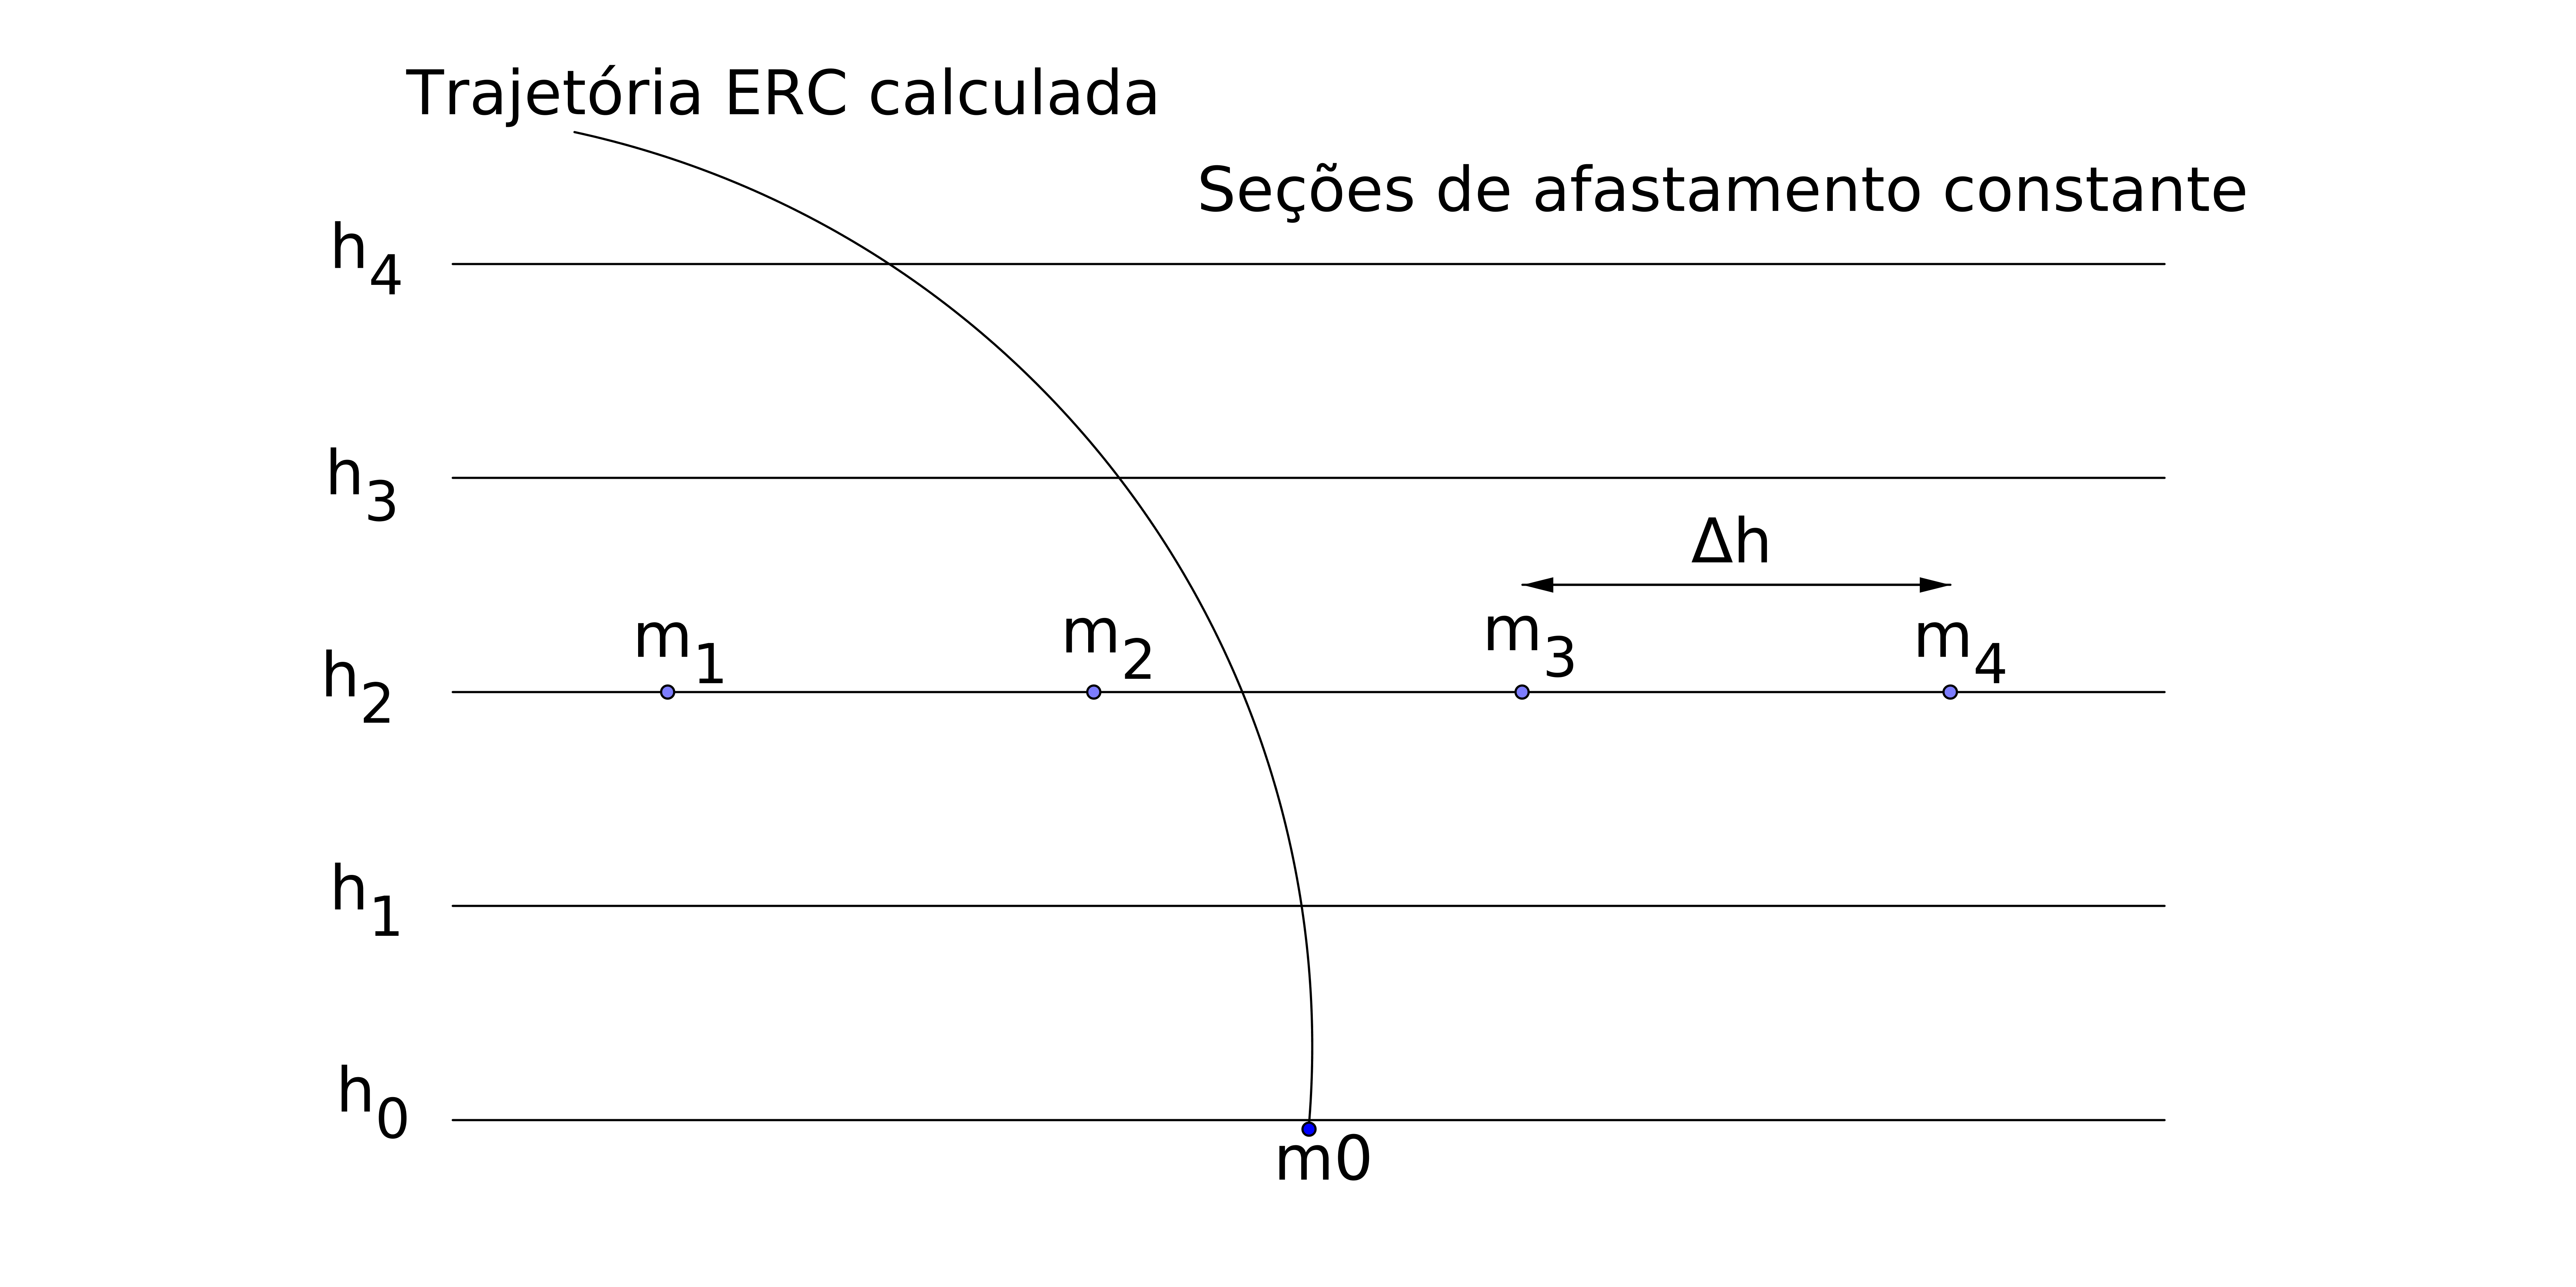
\includegraphics[scale=0.15]{images/interpolacao0.png}
\vspace{-0.3cm}
\end{center}
\begin{center}
 Fonte: Do Autor.
\end{center}
\label{fig:4.1}
\end{figure}


\begin{figure}
\caption{Representação esquemática das seções de afastamento constante após a interpolação. A discretização foi aumentada
intercalando traços zerados $m'_i$ entre os traços originais e depois realizando a interpolação FPE. O traço sísmico 
identificado pela coordenada $m'_2, h2$ está mais próximo da coordenada real da trajetória ERC calculada que os traços 
originais $m_2, h2$ e $m_3, h2$. o processo de interpolação é repetido até que a discretização seja suficiente para amostrar a 
trajetória ERC.}
\begin{center}
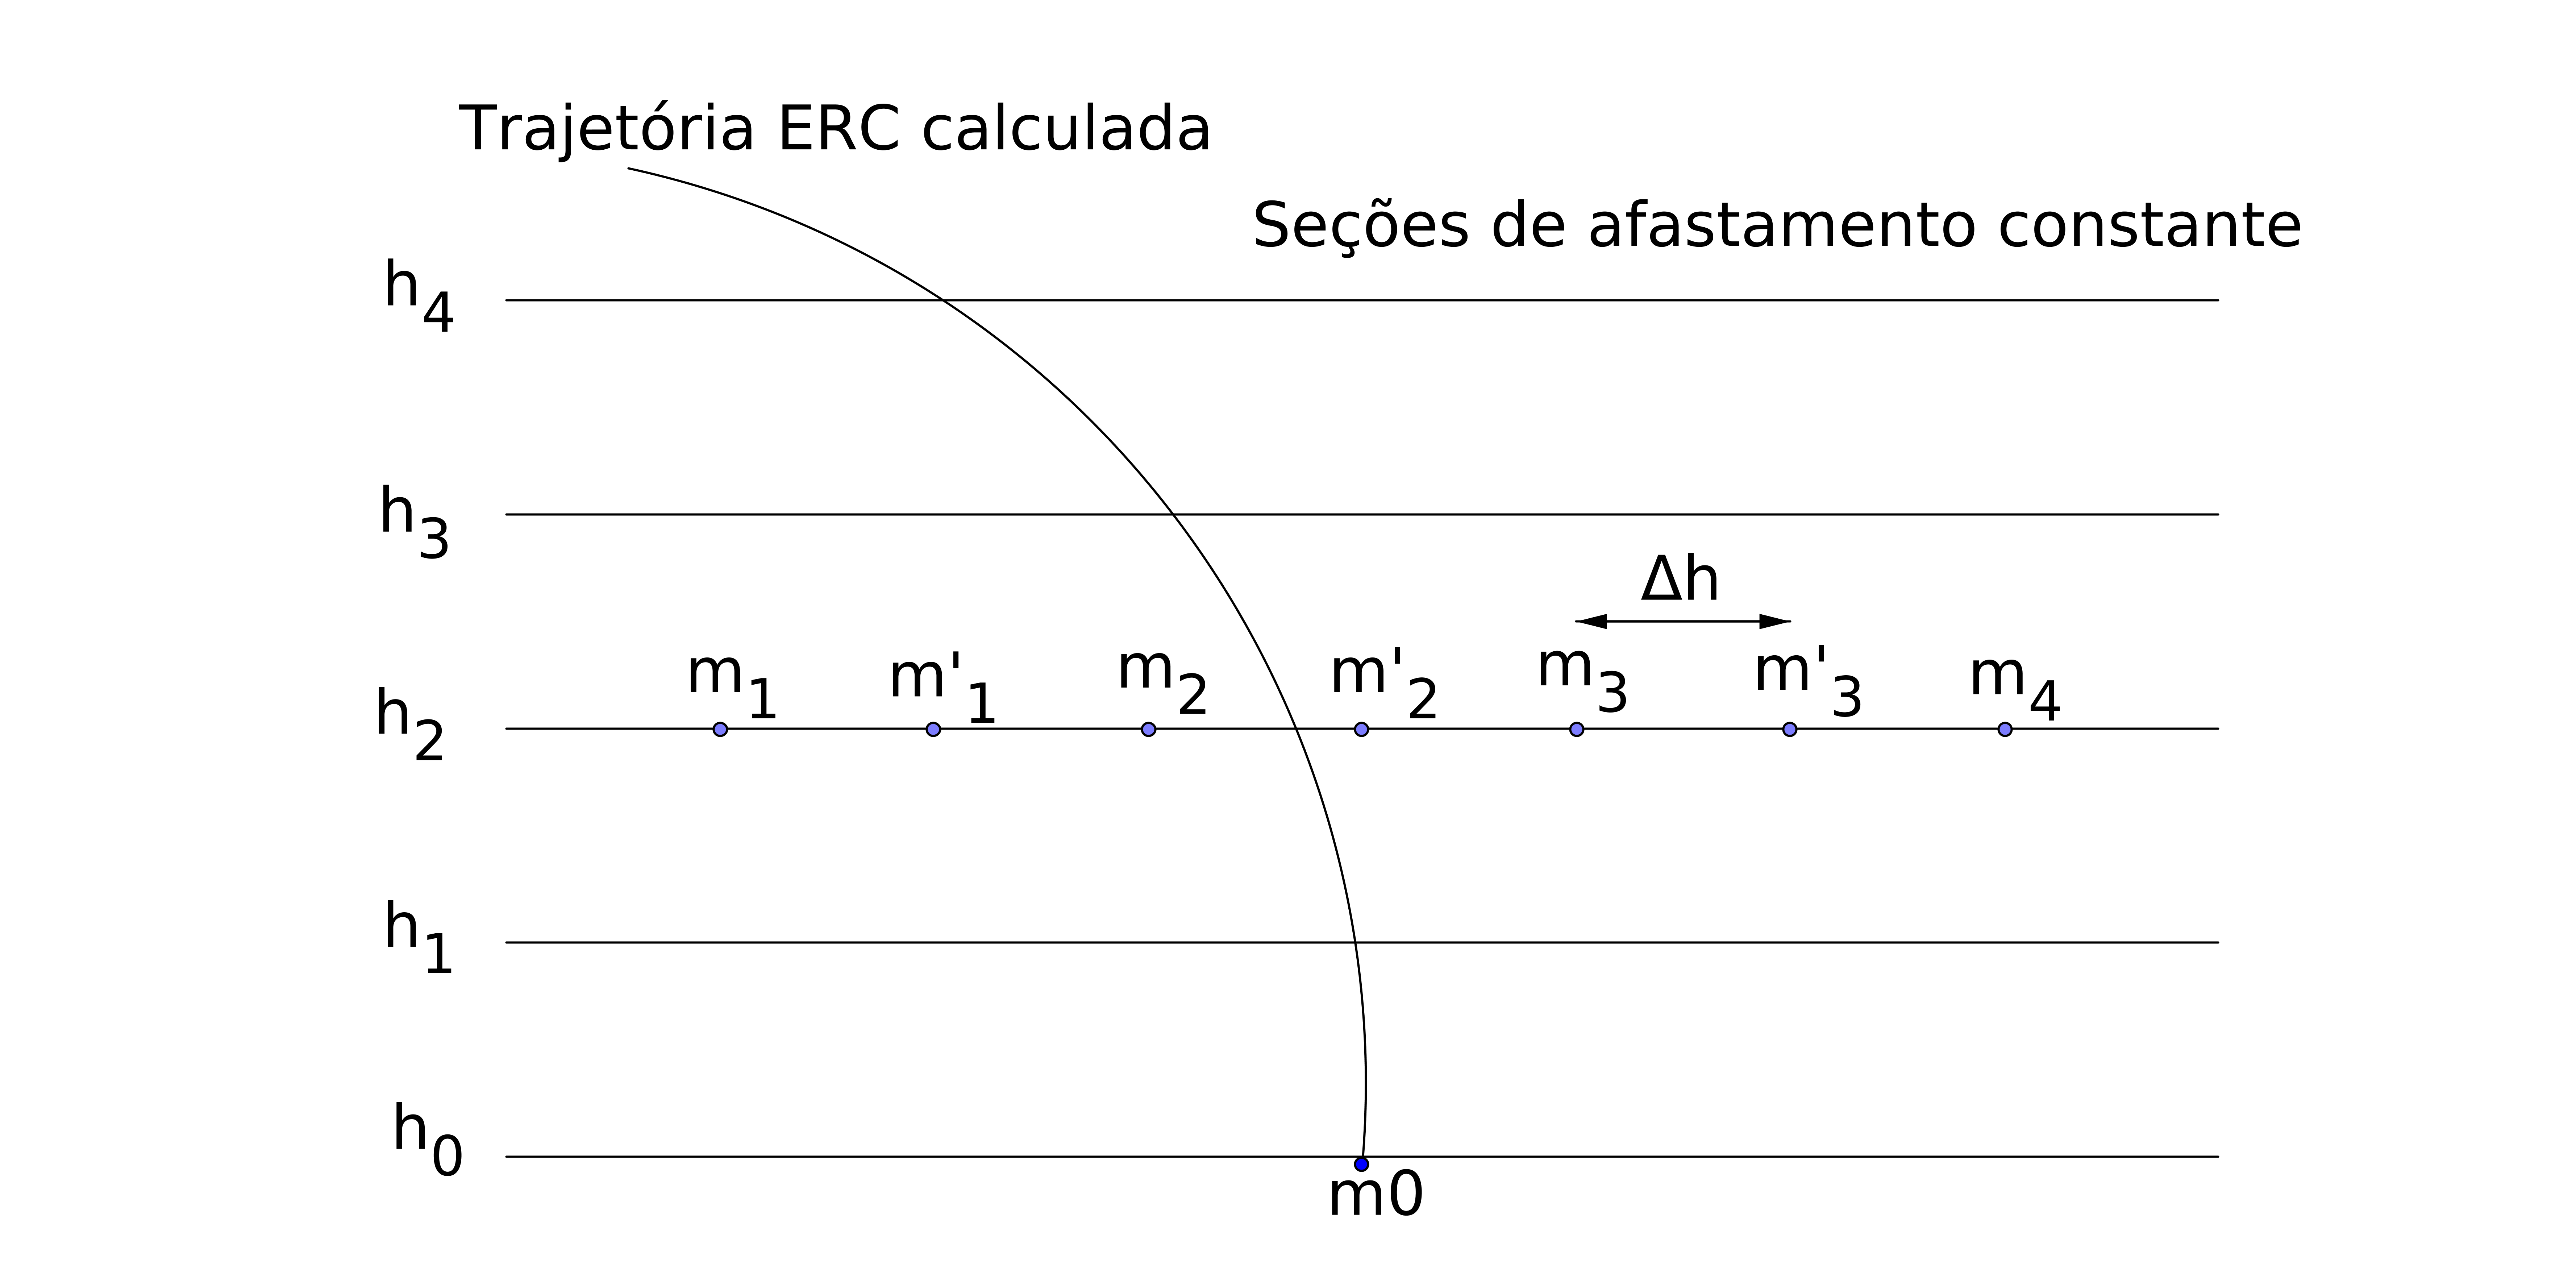
\includegraphics[scale=0.15]{images/interpolacao.png}
\vspace{-0.3cm}
\end{center}
\begin{center}
 Fonte: Do Autor.
\end{center}
\label{fig:4.2}
\end{figure}

 % Teoria intepolação com filtros PEF
%
% modeling.tex (LateX)
% 
% Objetivo: Capítulo sobre a etapa de modelagem do relatório de qualificação de doutorado.
% 
% Versão 1.0
% 
% Site: http://www.dirackslounge.online
% 
% Programador: Rodolfo A. C. Neves (Dirack) 16/10/2019
% 
% Email: rodolfo_profissional@hotmail.com
% 
% Licença: GPL-3.0 <https://www.gnu.org/licenses/gpl-3.0.txt>.

\chapter{MODELAGEM: REFLETOR GAUSSIANO EM UM MEIO COM GRADIENTE LINEAR DE VELOCIDADE}
\label{cap:modelagem}

Geramos uma superfície de tempo de trânsito de reflexão para o modelo do refletor gaussiano (Figura \ref{fig:5.1})
através da modelagem Kirchhoff\footnote{Este experimento é um dos vários ``artigos reproduzíveis'' disponíveis no site
do pacote de processamento sísmico Madagascar em \url{http://www.ahay.org/wiki/Main_Page}. 
Foi originalmente concebido por Sergey Fomel e Roman Kazinnik (2013),
está disponível para ser reutilizado sobre a licensa de uso GPL-3.0 para software livre disponível
em \url{https://www.gnu.org/licenses/gpl-3.0.txt}.}\cite{fomel1}.
Neste modelo a velocidade cresce linearmente com a profundidade com o gradiente 0.5, partindo da velocidade inicial de
1.5Km/s. 

A modelagem é realizada diretamente no domínio do ponto médio comum x afastamento. São 161 receptores (161 afastamentos),
espaçados de 0.025Km; e 401 PMC's, espaçados em 0.025Km. A frequência pico da wavelet é 10Hz, com 1001 amostras no tempo, a
cada 0.004s.

A Figura \ref{fig:5.2} apresenta os dados modelados organizados em um ``cubo de dados'' (as amplitudes nas amostras registradas
são identificadas pela tripla PMC, afastamento e tempo). A Figura \ref{fig:5.3} apresenta o tempo de trânsito de reflexão para o
modelo do refletor gaussiano, em função do PMC e do afastamento, em um mapa chamado de ``superfície de tempo de trânsito''.

Os menores tempos de reflexão são os registrados próximo ao 
ápice da gaussiana em 5Km (tempos em azul na Figura \ref{fig:5.3}) pela maior proximidade com o refletor.
E por último apresentamos a seção de afastamento nulo (Figura \ref{fig:5.4}) para o mesmo modelo.

\begin{figure}[H]
\caption{Modelo de velocidades utilizado na modelagem Kirchhoff: Modelo do refletor gaussiano em um meio com
gradiente linear de velocidade (a velocidade cresce linearmente com a profundidade). A velocidade próximo 
a superfície do modelo é 1.5Km/s e o gradiente de velocidade é 0.5.}
\begin{center}
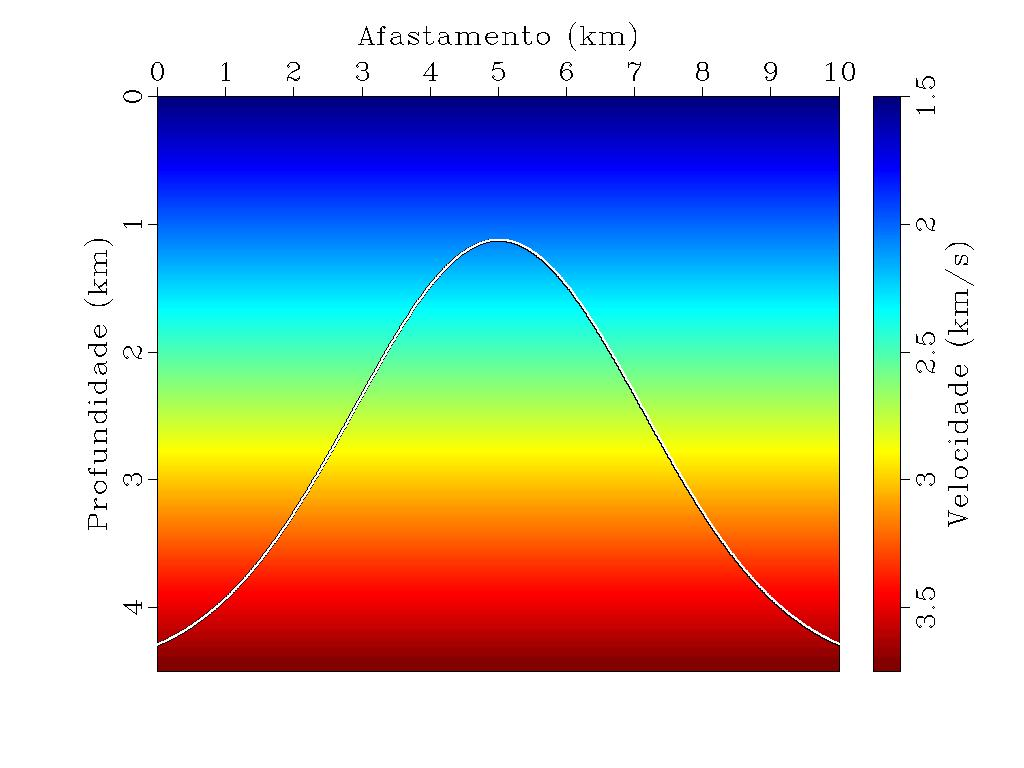
\includegraphics[scale=0.3]{images/dome.jpeg}
\vspace{-0.3cm}
\end{center}
\begin{center}
 Fonte: Do Autor.
\end{center}
\label{fig:5.1}
\end{figure}

\begin{figure}[htb]
\caption{Cubo de dados sísmicos modelados a partir da aplicação da modelagem Kirchoff ao modelo
do refletor gaussiano. O cubo apresenta os valores das amplitudes registradas em função das coordenadas do
ponto médio comum (PMC), afastamento e tempo.}
\begin{center}
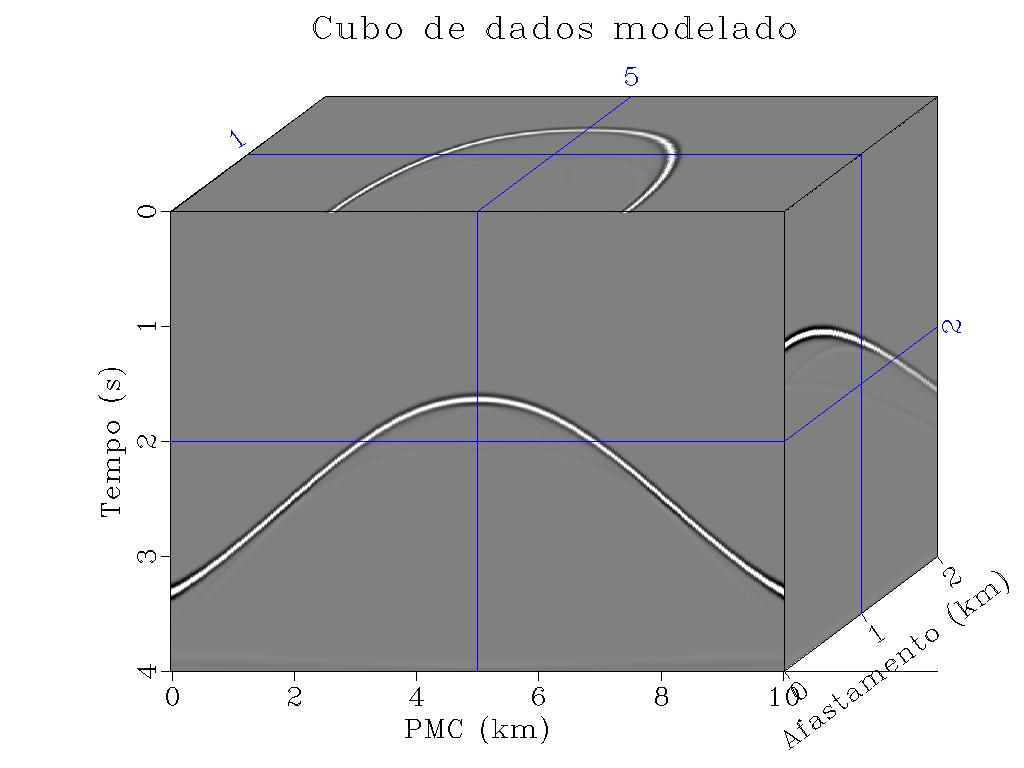
\includegraphics[scale=0.3]{images/dataCube.jpeg}
\vspace{-0.3cm}
\end{center}
\begin{center}
 Fonte: Do Autor.
\end{center}
\label{fig:5.2}
\end{figure}


%% Imagens dos offset gathers
\begin{figure}[htb]
\caption{Seção de afastamento constante extraída do cubo de dados. Esta seção representa um corte no
afastamento 0.5Km.}
\begin{center}
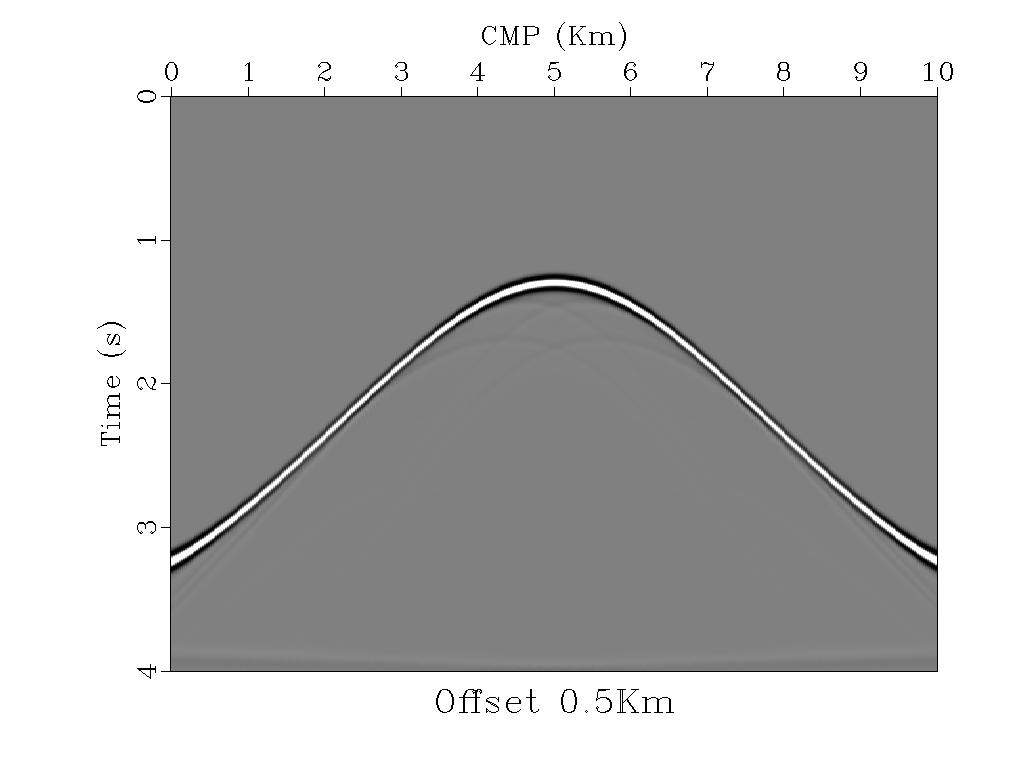
\includegraphics[scale=0.3]{images/off-40.jpeg}
\vspace{-0.3cm}
\end{center}
\begin{center}
 Fonte: Do Autor.
\end{center}
\label{fig:5.3}
\end{figure}

\begin{figure}[htb]
\caption{Seção de afastamento constante extraída do cubo de dados. Esta seção representa um corte no
afastamento 1.0Km.}
\begin{center}
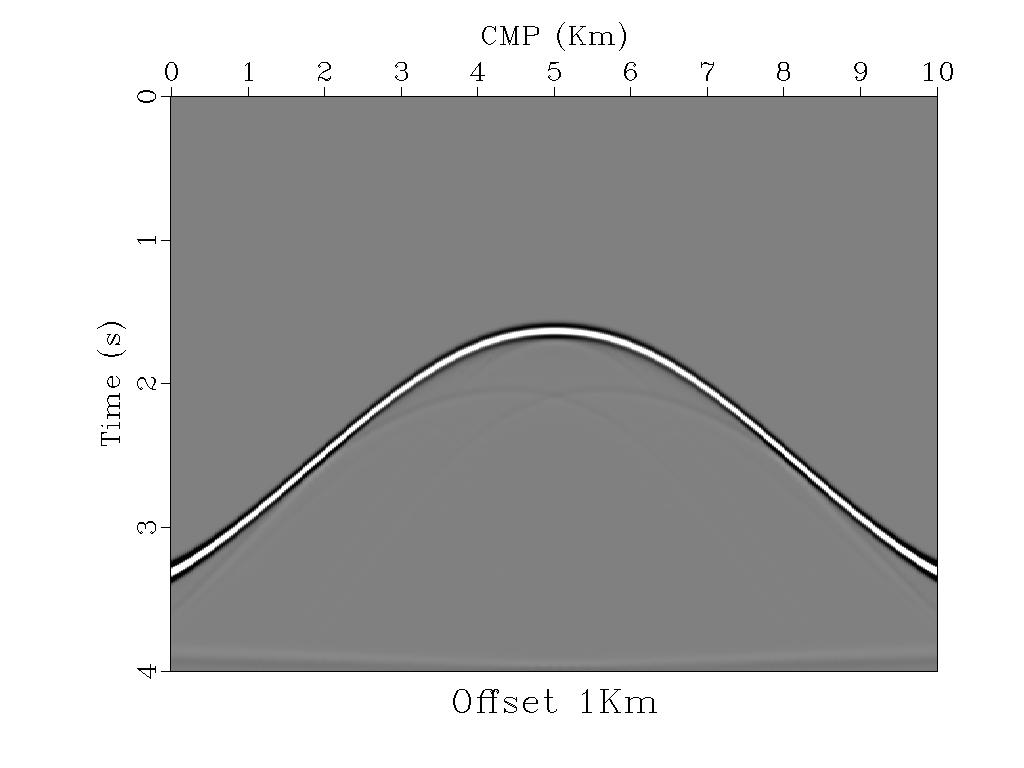
\includegraphics[scale=0.3]{images/off-80.jpeg}
\vspace{-0.3cm}
\end{center}
\begin{center}
 Fonte: Do Autor.
\end{center}
\label{fig:5.4}
\end{figure}

\begin{figure}[htb]
\caption{Seção de afastamento constante extraída do cubo de dados. Esta seção representa um corte no
afastamento 1.5Km.}
\begin{center}
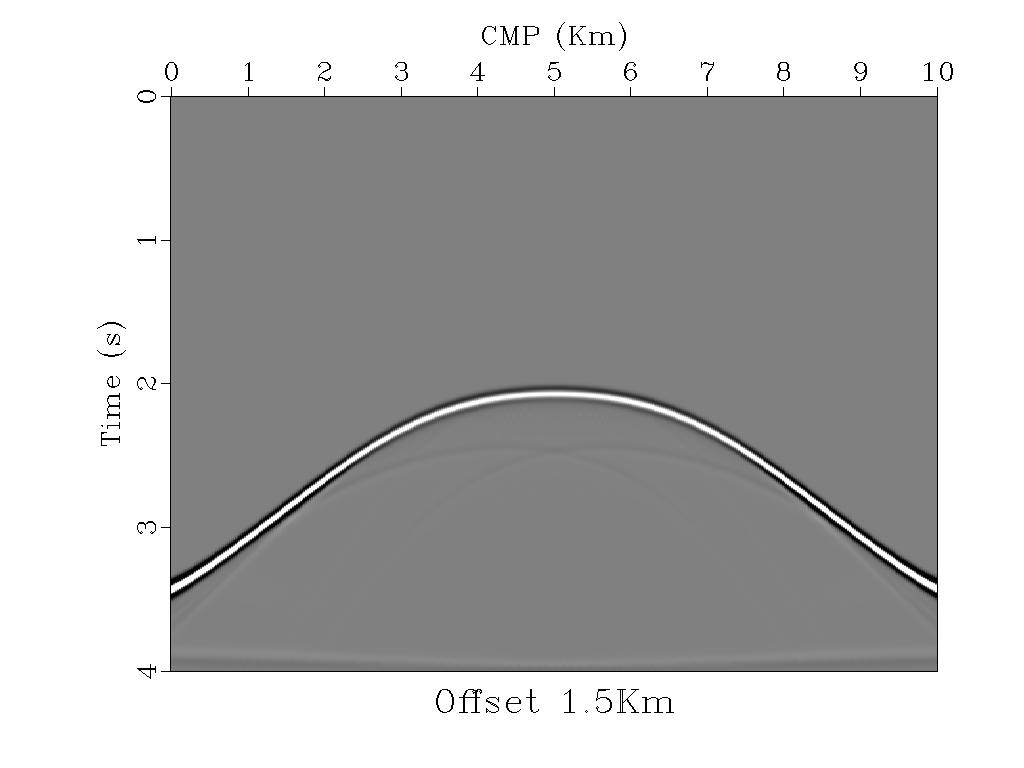
\includegraphics[scale=0.3]{images/off-120.jpeg}
\vspace{-0.3cm}
\end{center}
\begin{center}
 Fonte: Do Autor.
\end{center}
\label{fig:5.5}
\end{figure}



\begin{figure}[htb]
\caption{superfície de tempo de trânsito de reflexão para o modelo do refletor gaussiano.
O mapa apresenta os valores de tempo de trânsito registrados em função das coordenadas do
ponto médio comum (PMC) e afastamento.}
\begin{center}
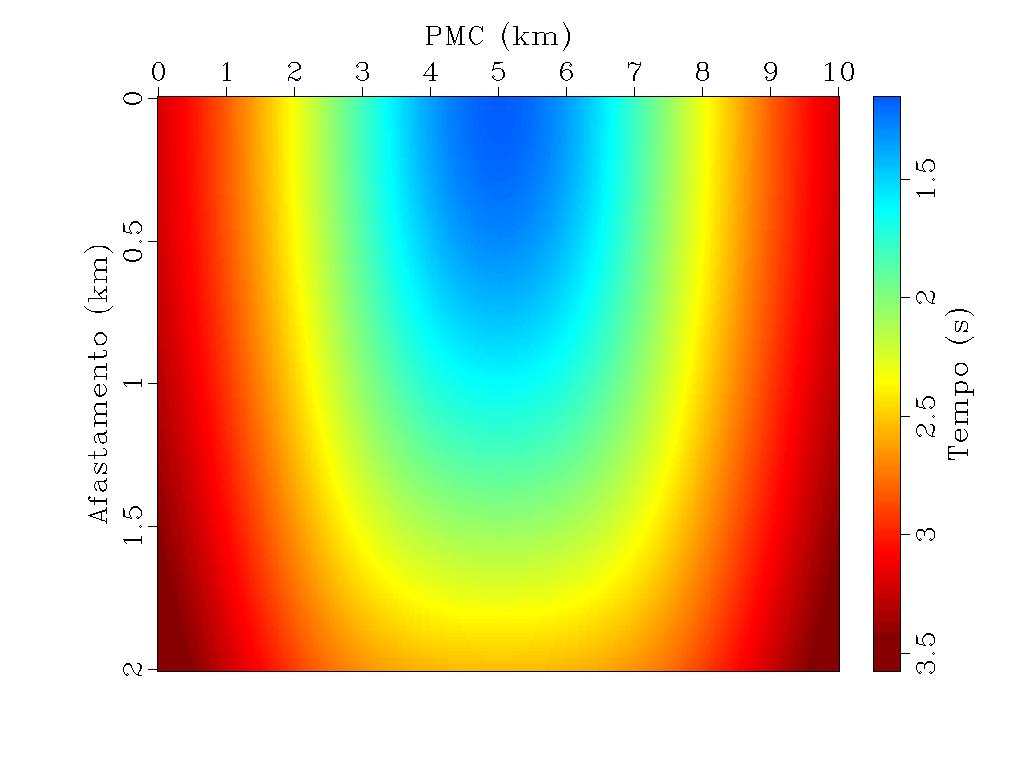
\includegraphics[scale=0.3]{images/reflectionSurface.jpeg}
\vspace{-0.3cm}
\end{center}
\begin{center}
 Fonte: Do Autor.
\end{center}
\label{fig:5.6}
\end{figure}

\begin{figure}[htb]
\caption{Seção de afastamento nulo para o modelo do refletor gaussiano.
A seção apresenta as amplitudes registradas em função das coordenadas do
ponto médio comum (PMC) e do tempo.}
\begin{center}
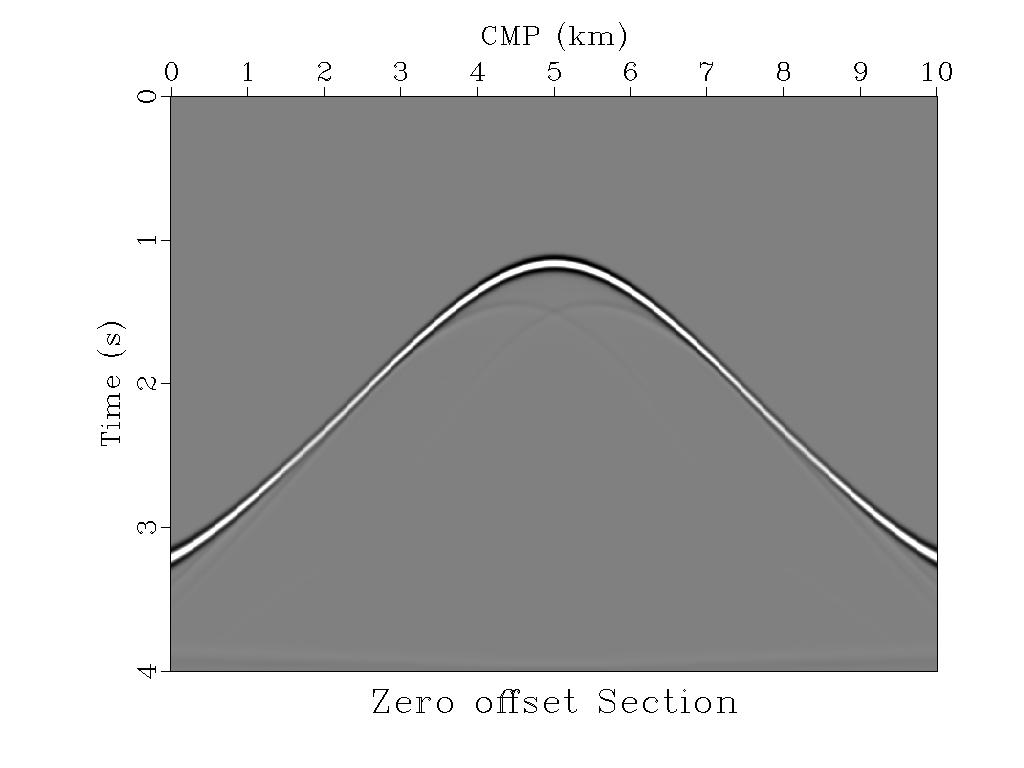
\includegraphics[scale=0.3]{images/zeroOffset.jpeg}
\vspace{-0.3cm}
\end{center}
\begin{center}
 Fonte: Do Autor.
\end{center}
\label{fig:5.7}
\end{figure}
 % Resultado da modelagem
%
% interpolacao.tex (LateX)
% 
% Objetivo: Capítulo sobre a etapa de interpolação do relatório de qualificação de doutorado.
% 
% Versão 1.0
% 
% Site: http://www.dirackslounge.online
% 
% Programador: Rodolfo A. C. Neves (Dirack) 17/10/2019
% 
% Email: rodolfo_profissional@hotmail.com
% 
% Licença: GPL-3.0 <https://www.gnu.org/licenses/gpl-3.0.txt>.

\chapter{INTERPOLAÇÃO COM FILTROS ADAPTATIVOS DE PREDIÇÃO DE ERRO}

A etapa de intepolação permite aumentar a amostragem dos dados modelados, de 0.025Km no afastamento, para 0.0125Km.
Isto é importante para montar as seções ERC, com os traços cujas coordenadas $m$ e $h$ estão o mais próximo possível
das coordenadas $m$, $h$ da curva ERC calculada.

Obviamente, poderíamos ter realizado a etapa de modelagem com uma discretização maior, porém o intuito é mostrar como
a intepolação com filtros de erro adaptativos pode regularizar a amostragem dos dados, possibilitando a busca pelos
traços que estão sobre as trajetórias ERC com a maior precisão possível.

Antes da interpolação, os dados sísmicos nas coordenadas $m$ e $h$ são separados em seções de afastamento constante.
A interpolação com os filtros adaptativos de predição de erro (FPE) é realizada para cada seção, aumentando assim a
sua discretização (de 0.025Km para 0.0125Km). Após esta etapa, calculamos as trajetórias ERC para cada $m0$, e determinamos
as coordenada $m$, $h$ dos pontos sobre estas trajetórias que intersectam as seções de afastamento constante. Estes pontos
$m$, $h$ serão as coordendas dos traços que pertencem à trajetória ERC, por definição.

Com o conhecimento das coordenadas $m$, $h$ dos traços sobre a ERC, determinados anteriormente, buscamos nas seções interpoladas
os traços sísmicos com as coordenadas $m$ e $h$ mais próximas das trajetórias ERC calculadas, e montamos as seções ERC. 
Cada PMC $m0$ possuirá uma seção ERC e parâmetros $R_N$, $R_{NIP}$ e $\beta_0$; e cada par $m0$, $t0$ terá uma curva de tempo
de trânsito ERC correspondente. O empilhamento ERC é realizado sobre as curvas de tempo de trânsito ERC,, somando as amplitudes
das amostras sobre a curva e atribuindo esta soma aos pares $m0$, $t0$ na seção empilhada ERC.

A Figura \ref{fig:6.1}-\ref{fig:6.2} apresentam as seções ERC organizadas pela coordenada do afastamento $h$. A Figura
\ref{fig:6.1} é a seção ERC para o $m0=5Km$ e as Figuras \ref{fig:6.2}-\ref{fig:6.3} para o $m0=4Km$. O ajuste feito com
a equação de tempo de trânsito ERC (pontos em amarelo) depende também da escolha do tempo $t0$. Na Figura \ref{fig:6.3}, 
o $t0=1.1s$ utilizado não é apropriado, não produzindo o melhor ajuste. Portanto, o empilhamento sobre as curvas que possuam
os melhores ajustes com os dados modelados tendem a produzir somas construtivas, enquanto o empilhamento sobre curvas de
pior ajuste, tendem a produzir somas destrutivas.

\begin{figure}
\caption{Seção CRE para o PMC $m0=5Km$ e $t0=1.1s$.
Pontos em amarelo representa a curva de tempo de trânsito ERC sobre a qual
será realizado o empilhamento ERC.
O eixo horizontal é a coordenada do afastamento $h$ e o eixo vertical o tempo
$t$.}
\begin{center}
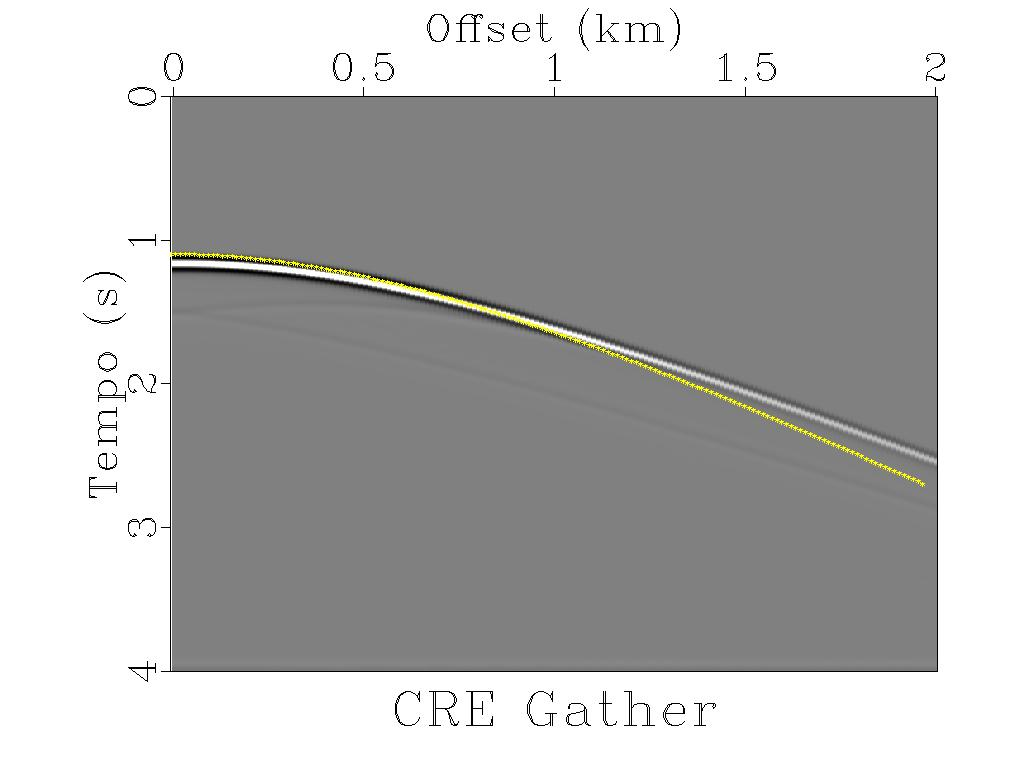
\includegraphics[scale=0.3]{images/interpolacao5.jpeg}
\vspace{-0.3cm}
\end{center}
\begin{center}
 Fonte: Do Autor.
\end{center}
\label{fig:6.1}
\end{figure}

\begin{figure}
\caption{Seção CRE para o PMC $m0=4Km$ e $t0=1.3s$.
Pontos em amarelo representa a curva de tempo de trânsito ERC sobre a qual
será realizado o empilhamento ERC.
O eixo horizontal é a coordenada do afastamento $h$ e o eixo vertical o tempo
$t$.}
\begin{center}
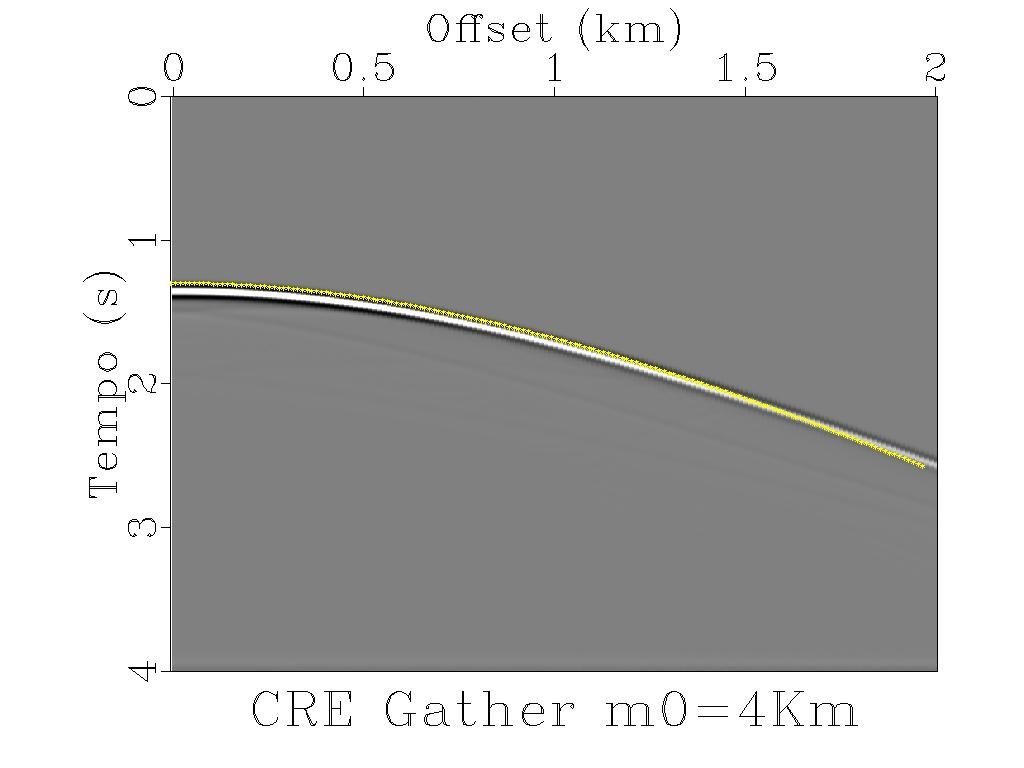
\includegraphics[scale=0.3]{images/interpolacao4.jpeg}
\vspace{-0.3cm}
\end{center}
\begin{center}
 Fonte: Do Autor.
\end{center}
\label{fig:6.2}
\end{figure}

\begin{figure}
\caption{Seção CRE para o PMC $m0=4Km$ e $t0=1.1s$.
Pontos em amarelo representa a curva de tempo de trânsito ERC sobre a qual
será realizado o empilhamento ERC.
O eixo horizontal é a coordenada do afastamento $h$ e o eixo vertical o tempo
$t$. A escolha de $t0=1.1$ não produziu o melhor ajuste da curva ERC aos dados modelados.}
\begin{center}
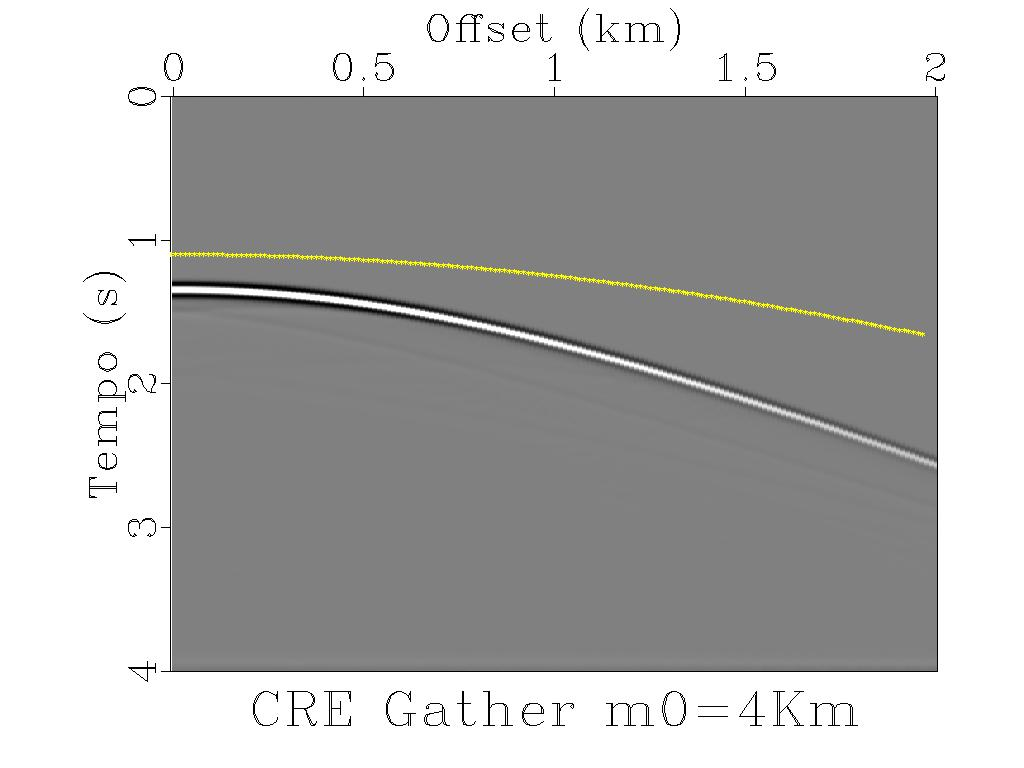
\includegraphics[scale=0.3]{images/interpolacaoErro.jpeg}
\vspace{-0.3cm}
\end{center}
\begin{center}
 Fonte: Do Autor.
\end{center}
\label{fig:6.3}
\end{figure}
 % Resultados da Interpoção com PEF
%
% empilhamento.tex (LateX)
% 
% Objetivo: Capítulo sobre a etapa de modelagem do relatório de qualificação de doutorado.
% 
% Versão 1.0
% 
% Site: http://www.dirackslounge.online
% 
% Programador: Rodolfo A. C. Neves (Dirack) 17/10/2019
% 
% Email: rodolfo_profissional@hotmail.com
% 
% Licença: GPL-3.0 <https://www.gnu.org/licenses/gpl-3.0.txt>.

\chapter{EMPILHAMENTO FAMÍLIAS ERC}
\label{cap:empilhamento}

O empilhamento ERC foi realizado após a interpolação com filtros adaptativos de predição de erro (FPE). Esta etapa de
interpolação permite amostrar a trajetória de tempo de trânsito ERC com um intervalo de amostragem satisfatório no
domínio do PMC. O empilhamento ERC é feito nas famílias ERC sobre as trajtórias de tempo de trânsito ERC. Cada ponto sobre
a seção empilhada ERC ($m_0$,$t_0$) corresponderá a uma família ERC e a uma trajetória ERC, 
o resultado do empilhamento no domínio
ERC é atribuído à coordenada $m_0$,$t_0$ na seção empilhada ERC, formando a imagem na seção empilhada.

Para demonstrar o funcionamento do empilhamento ERC, selecionamos um único traço na coordenada $m_0=4Km$ no modelo do refletor
gaussiano no Capítulo \ref{cap:modelagem}. O espectro de amplitude deste traço é apresentado na Figura \ref{fig:7.1}, o máximo valor de amplitude 
está na frequência 10Hz e corresponde a frequência pico da wavelet utilizada.


Foi realizada a interpolação FPE para o cubo de dados do modelo do refletor gaussiano (vide Capítulo \ref{cap:modelagem}),
aumentando a amostragem
do modelo na corrdenada do PMC para 802 PMC's, e diminuindo a discretização para 0.0125Km também no domínio PMC. O processo 
de interpolação seleciona as seções de afastamento constante no cubo de dados, intercala os traços originais da seção com traços 
zerados e interpola os traços intercalados utilizando a informação dos traços originais. Este processo é feito para cada seção
de afastamento constante selecionada, regularizando todo o cubo de dados.

Para obter o supertraço empilhado do PMC escolhido ($m_0=4Km$) é escolhida uma janela de tempo $0<t_0<1s$, 
e para cada par $m_0,t_0$
são calculados os parâmetros do SRC de afastamento nulo $R_{NIP}$ e $\beta_0$ através da otimização global com o Very Fast
Simulated Aneeling (VFSA). Após a obtenção dos parâmetros ótimos, deteminamos as coordenadas $m,h$ que fazem parte da trajetória ERC
e buscamos no cubo de dados interpolados os traços que estão sobre esta trajetória, estes formam uma família ERC.

Os parâmetros $R_{NIP}$ e $\beta_0$ também permitem calcular uma trajetória de empilhamento no domínio ERC, esta será utilizada
para empilhar as amostras sobre esta curva na família ERC correspondente a uma coordenada $m_0, t_0$ da seção empilhada.
Cada $m_0$ constante corresponde a um supertraço da seção empilhada ERC. 

A Figura \ref{fig:7.2} apresenta o resultado do empilhamento para o supertraço $m_0=4Km$. O supertraço apresenta ruído numérico
proveninte dos processos de interpolação e empilhamento, para atenuar este ruído utilizamos um filtro banda-passante no 
intervalo de 0Hz a 10Hz. O resultado, após a aplicação do filtro, é apresentado na Figura \ref{fig:7.4}. O espectro de amplitudes
do supertraço antes e depois da filtragem é apresentado nas Figuras \ref{fig:7.3} e \ref{fig:7.5}.

\begin{figure}
\caption{Espectro original do traço na seção de afastamento nulo com PMC 4Km.}
\begin{center}
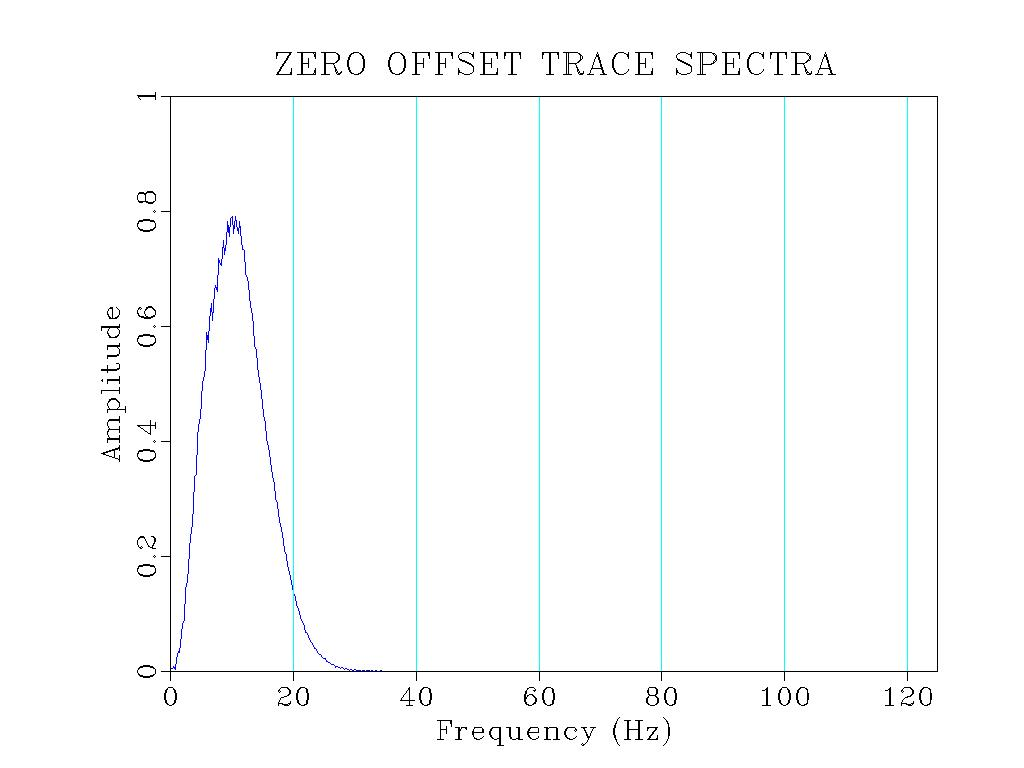
\includegraphics[scale=0.4]{images/originalTraceSpectra.jpeg}
\vspace{-0.3cm}
\end{center}
\begin{center}
 Fonte: Do Autor.
\end{center}
\label{fig:7.1}
\end{figure}


\begin{figure}
\caption{Resultado do empilhamento CRE: Supertraço para m0=4Km. A interpolação e o empilhamento cre adicionam
ruído numérico aos dados empilhados.}
\begin{center}
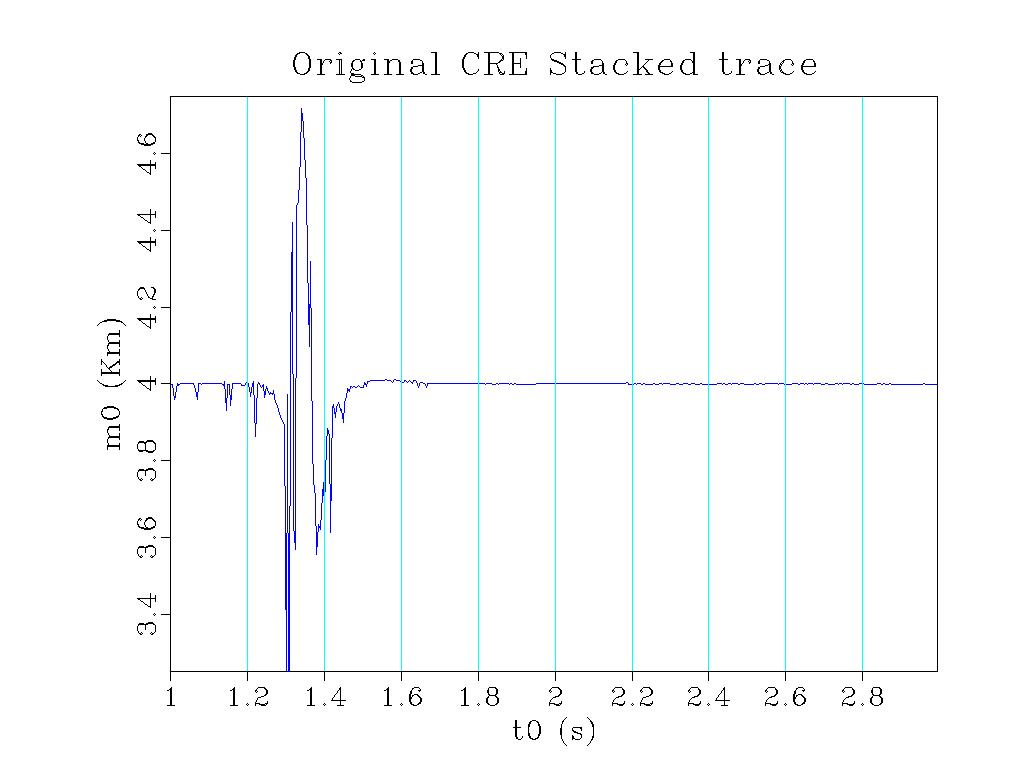
\includegraphics[scale=0.4]{images/creStackedSection.jpeg}
\vspace{-0.3cm}
\end{center}
\begin{center}
 Fonte: Do Autor.
\end{center}
\label{fig:7.2}
\end{figure}

\begin{figure}
\caption{Espectro de amplitude original do supertraço CRE para m0=4Km.}
\begin{center}
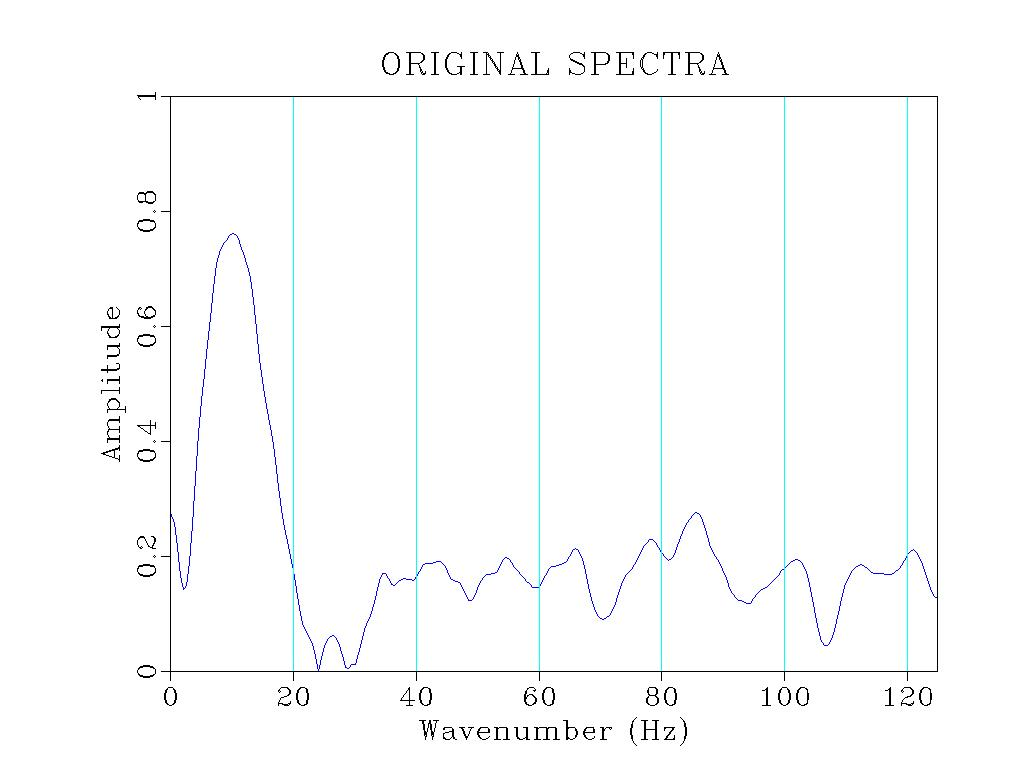
\includegraphics[scale=0.4]{images/originalSpectra.jpeg}
\vspace{-0.3cm}
\end{center}
\begin{center}
 Fonte: Do Autor.
\end{center}
\label{fig:7.3}
\end{figure}

\begin{figure}
\caption{Supertraço cre após a filtragem banda passante.}
\begin{center}
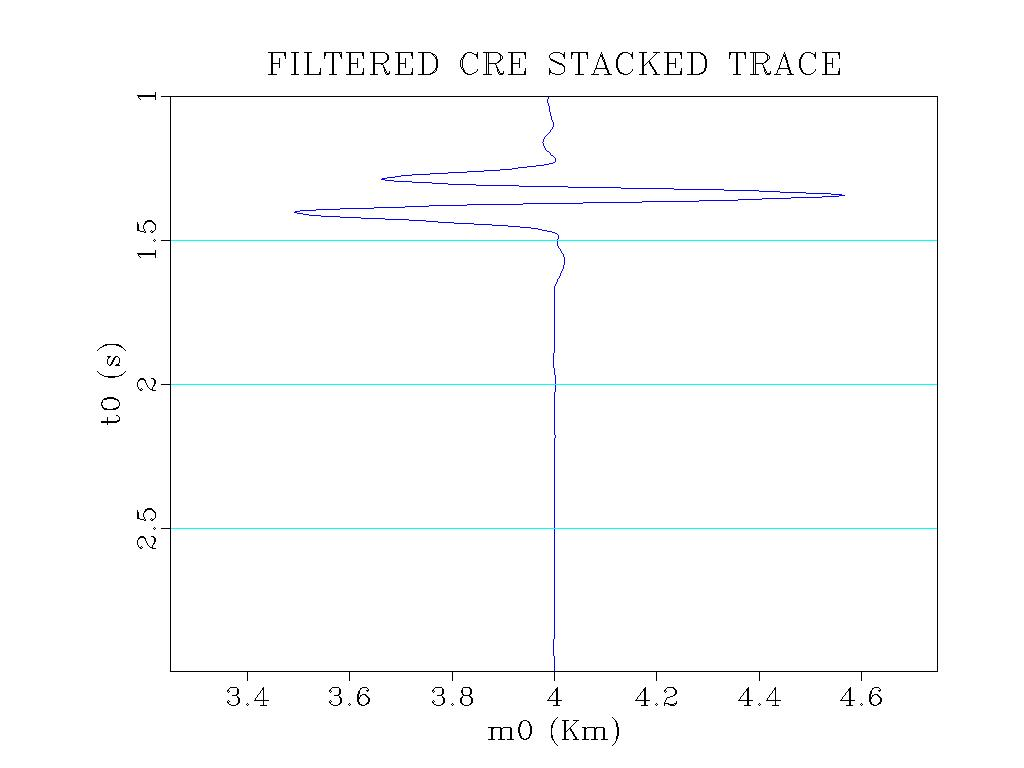
\includegraphics[scale=0.4]{images/creStackedSectionFiltered.jpeg}
\vspace{-0.3cm}
\end{center}
\begin{center}
 Fonte: Do Autor.
\end{center}
\label{fig:7.4}
\end{figure}

\begin{figure}
\caption{Espectro de amplitude após a filtragem banda passante.}
\begin{center}
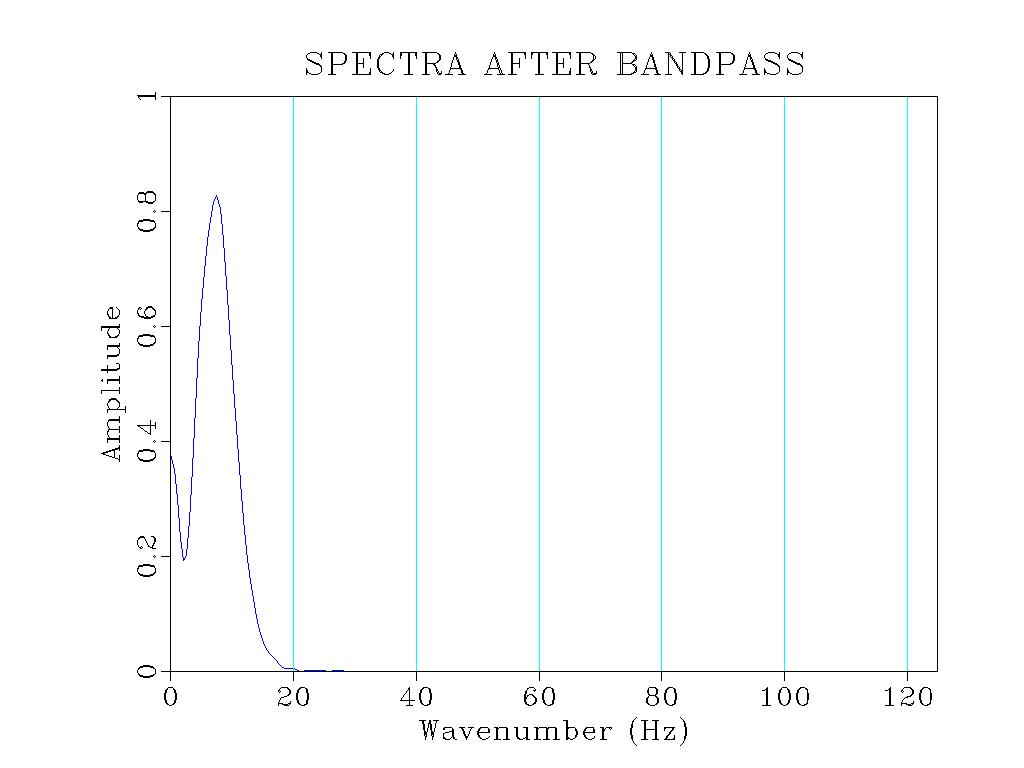
\includegraphics[scale=0.4]{images/filteredSpectra.jpeg}
\vspace{-0.3cm}
\end{center}
\begin{center}
 Fonte: Do Autor.
\end{center}
\label{fig:7.5}
\end{figure}

%% Figuras seção empilhada CRE com a equação de tempo de trânsito CRE

O empilhamento para um dado $m_0$, descrito acima, é realizado para um conjunto de $m_0's$ para formar a seção empilhada.
Cada $m_0$ será um supertraço da seção.
A amostragem entre os PMC's da seção empilhada é 0.0125Km, são 160 PMC's no intervalo de $4Km<m<5Km$. O eixo do tempo na 
seção é o tempo de trânsito do raio normal $t_0$ com $1s<t_0<1.5s$, com 125 amostras e amostragem no tempo de 0.004s.
Para comparação dos resultados do empilhamento, foi extraída a seção de afastamento nulo do cubo de dados do modelo do
refletor gaussiano (Figura \ref{fig:4.2} no Capítulo \ref{cap:modelagem}) apresentada na Figura \ref{fig:7.6}.

A Figura \ref{fig:7.7} é o resultado do empilhamento ERC utilizando a aproximação de tempo de trânsito ERC \ref{eq:2.3}
como trajetória de empilhamento. O empilhamento adicionou ruído numérico nos traços da seção, por isto foi realizada a filtragem
banda passante com a frequência máxima de corte em 20Hz. O resultado após a aplicação do filtro é apresentado na Figura
\ref{fig:7.8}.

O empilhamento também foi realizado com auxílio da aproximação de tempo de trânsito SRC não hiperbólica aplicando a condição CDS
($R_N=R_{NIP}$). Aplicada esta condição, a curva de tempo de trânsito SRC foi utilizada como trajetória de empilhamento no domínio
ERC, o resultado é apresentado na Figura \ref{fig:7.9}. Também foi realizada a aplicação da filtragem banda passante na seção
empilhada com a aproximação do SRC não hiperbólico, a frequência máxima de corte utilizada foi 20Hz, o resultado é apresentado
na Figura \ref{fig:7.10}.

\begin{figure}
\caption{Seção zero offset extraída do cubo de dados.}
\begin{center}
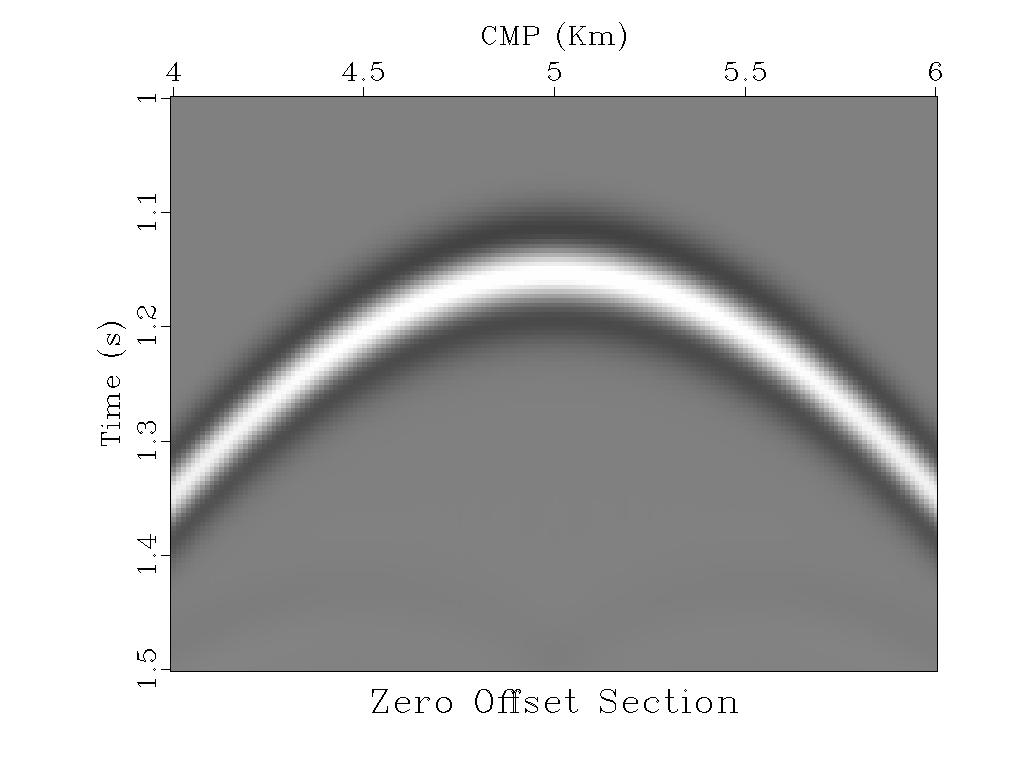
\includegraphics[scale=0.4]{images/zeroOffsetSection.jpeg}
\vspace{-0.3cm}
\end{center}
\begin{center}
 Fonte: Do Autor.
\end{center}
\label{fig:7.6}
\end{figure}

\begin{figure}
\caption{Seção empilhada ERC bruta.}
\begin{center}
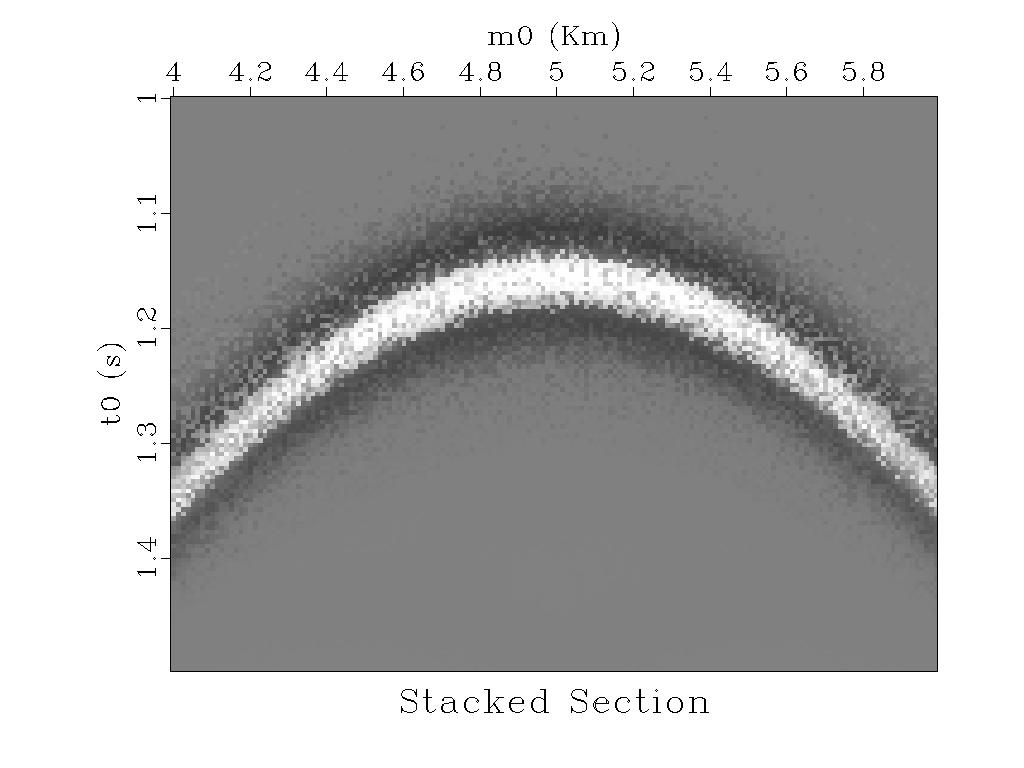
\includegraphics[scale=0.4]{images/stackedSection.jpeg}
\vspace{-0.3cm}
\end{center}
\begin{center}
 Fonte: Do Autor.
\end{center}
\label{fig:7.7}
\end{figure}

\begin{figure}
\caption{Seção empilhada ERC após filtragem de banda passante (Corte em 20Hz).}
\begin{center}
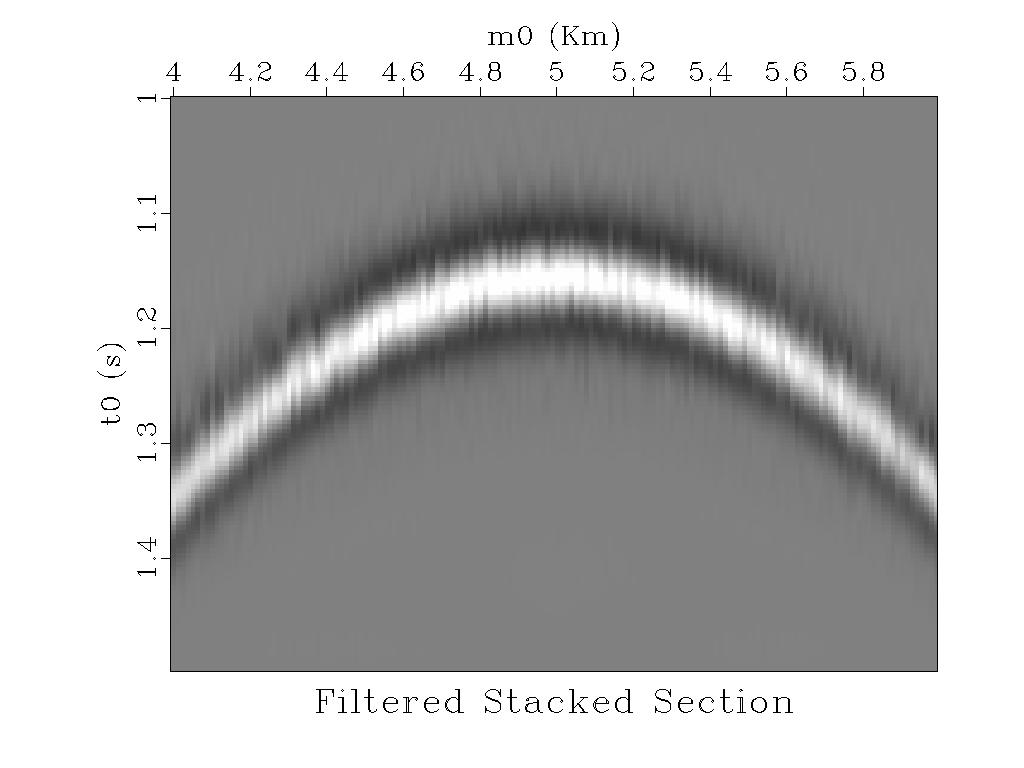
\includegraphics[scale=0.4]{images/filteredStackedSection.jpeg}
\vspace{-0.3cm}
\end{center}
\begin{center}
 Fonte: Do Autor.
\end{center}
\label{fig:7.8}
\end{figure}

%% Figuras Empilhamento CRS não hiperbólico
\begin{figure}
\caption{Seção empilhada ERC bruta produzida a partir do empilhamento sobre a curva de tempo de trânsito SRC não hiperbólica
utilizando a condição CDS ($R_N=R_{NIP}$).}
\begin{center}
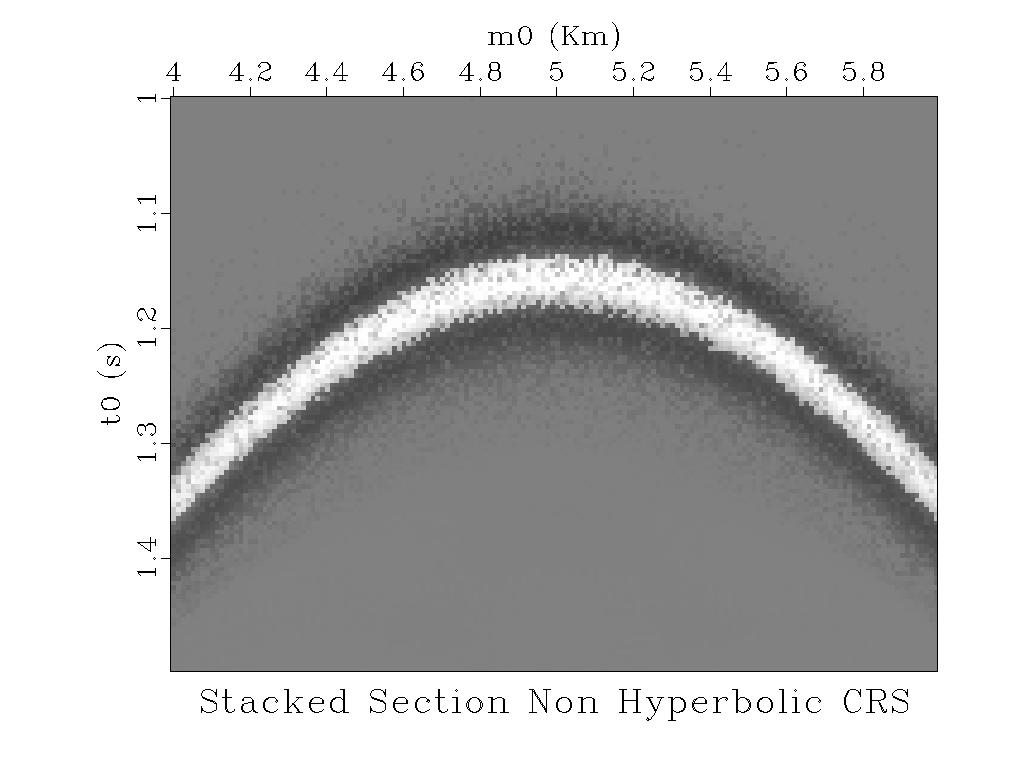
\includegraphics[scale=0.4]{images/stackedSectionNcrs.jpeg}
\vspace{-0.3cm}
\end{center}
\begin{center}
 Fonte: Do Autor.
\end{center}
\label{fig:7.9}
\end{figure}

\begin{figure}
\caption{Seção empilhada ERC após filtragem de banda passante (Corte em 20Hz) produzida a partir do empilhamento 
sobre a curva de tempo de trânsito SRC não hiperbólica
utilizando a condição CDS ($R_N=R_{NIP}$).}
\begin{center}
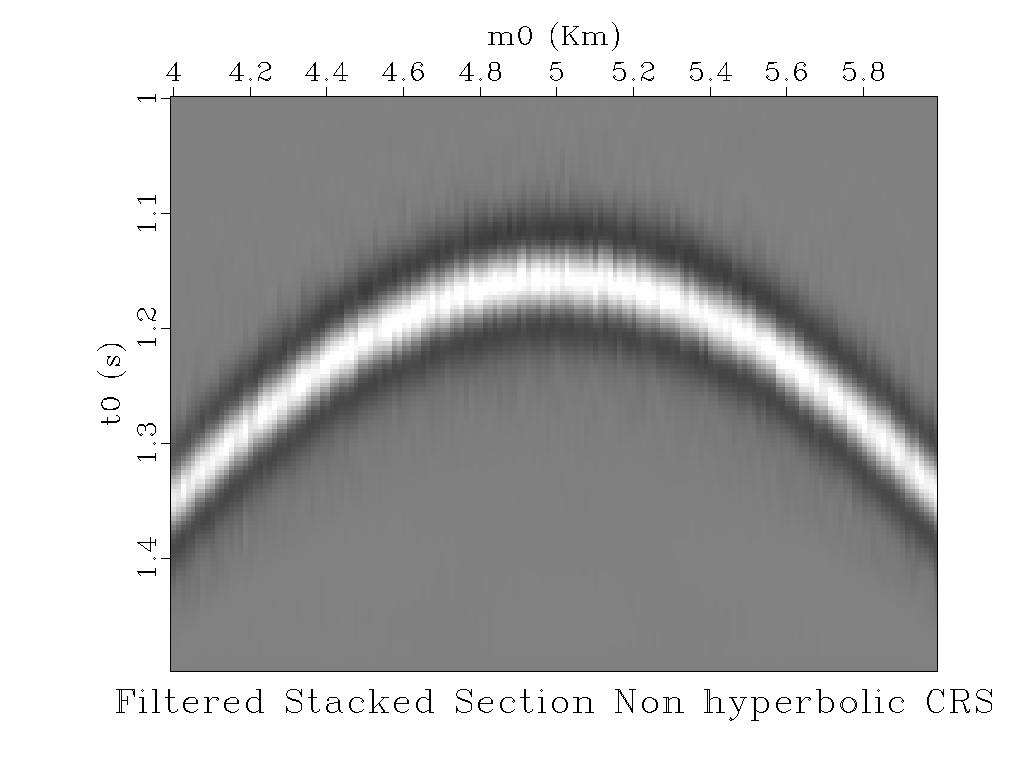
\includegraphics[scale=0.4]{images/filteredStackedSectionNcrs.jpeg}
\vspace{-0.3cm}
\end{center}
\begin{center}
 Fonte: Do Autor.
\end{center}
\label{fig:7.10}
\end{figure}
 % Resultados do empilhamento cre
\chapter{INVERSÃO DO MODELO DE VELOCIDADES}
\label{cap8:velocidades}

Propomos a seguinte metodologia para a inversão do modelo de velocidades e cumprimento do objetivo da tese:
Utilizar a simulação de resposta de difrações com a aproximação de tempo de trânsito ERC (Equação \ref{eq:2.3}) ou
a aproximação de tempo de trânsito do SRC não hiperbólico (Equação \ref{eq:2.4}), 
com aplicação da condição SDC ($R_N=R_{NIP}$),
para simular as difrações \cite{diffractions}.

O conceito de determinação da velocidade através da simulação de resposta de difração
consiste dos seguintes passos \cite{diffractions}:

\begin{enumerate}
 \item Determinação da velocidade NMO: Isto pode ser feito em cascata nos pontos da
seção empilhada, camada por camada otimizando a velocidade uma camada por vez.
\item Determinação dos slopes de reflexão de afastamento nulo no cubo de dados empilhados: 
Este passo não será necessário na nova metodologia.
\item Transformação dos traços zero offset selecionados em respostas de pontos difratores em CDP's
selecionados.
\item Aplicação da migração em profundidade pós empilhamento com análise de velocidades
em looping.
\end{enumerate}

A partir da seção empilhada ERC transformamos cada par $m_0, t_0$ sobre um refletor em uma resposta simulada de
uma fonte pontual (Ponto difrator) na forma de hipérboles de difração. Escolhido um par $m_0, t_0$, ele terá um par
de parâmetros $R_{NIP}, \beta_0$ que possibilitam traçar uma hipérbole de difração a partir da aproximação do SRC
não hiperbólico utilizando a condição SDC ($R_N=R_{NIP}$).

Espalhando o valor de amplitude do ponto escolhido na seção empilhada $A(m_0,t_0)$ sobre a hipérbole de difração
previamente calculada, teremos a resposta simulada de uma difração \cite{diffractions}. A inversão do modelo de velocidades
se torna a busca pelas velocidades de migração que melhor focalizam as hipérboles de difração simuladas.

Depois realizaremos a análise de velocidades automatizada no domínio pós empilhado e o imageamento de alta resolução
para heterogeneidades de pequena escala produzindo imagens migradas no tempo com as hipérboles de difração
focalizadas. Este processo contará com a análise automatizada de focalização para a detecção das
velocidades de migração ótimas para imageamento das hipérboles de difração simuladas \cite{sep_dif}.

A migração será realizada a partir de um algoritmo de continuação de velocidades \cite{fomel2003a}, um método que performa
a análise de velocidade de migração em tempo continuando imagens sísmicas na velocidade, também chamado de
``ondas imagem'' \cite{hubral1996}. A teoria da continuação de velocidades mostra ser possível realizar a migração no tempo
com um conjunto de diferentes velocidades fazendo pequenos incrementos na velocidade diretamente no domínio da imagem.
Implementaremos através de um algoritmo baseado na tranformada rápida de Fourier \cite{bfomel2003}.

Aplicaremos uma medida de focalização local para obter os painéis de velocidade de migração para cada ponto no domínio da
imagem. E realizaremos a análise de velocidades automatizada, com a principal diferença de que a informação sobre a velocidade
será obtida da análise da medida de focalização das difrações ao invés da coerência \cite{sep_dif}.
Os resultados obtidos são as velocidades de migração que melhor focalizam as hipérboles da seção simulada e tangente as hipérboles
aparecerá a imagem do refletor.

\begin{figure}[htb]
\caption{Fluxograma do algoritmo de inversão do modelo de velocidades.}
\begin{center}
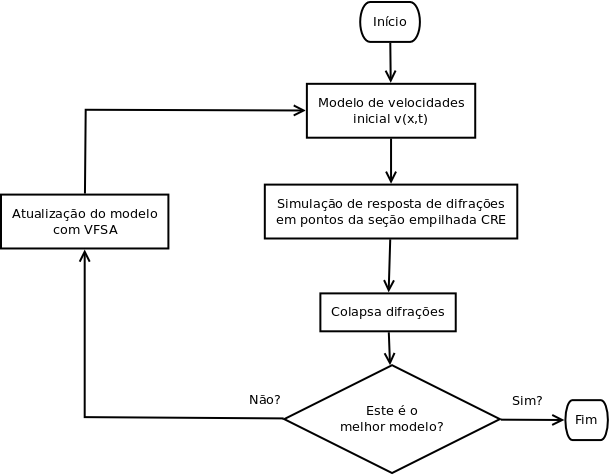
\includegraphics[scale=0.30]{images/fluxoVel.png}
\vspace{-0.3cm}
\end{center}
\begin{center}
 Fonte: Do Autor.
\end{center}
\label{fig:8.1}
\end{figure} % Proposta de uma metodologia para inversão do modelo de velocidades
\chapter{CRONOGRAMA}
\label{cap9:cronograma}


\section{Etapas concluídas}

A seguir a descrição das etapas concluídas e o cronograma:

  \begin{enumerate}
   \item  Pesquisa e fundamentação teórica: Pesquisa das principais referências e estabelecimento do tema central da tese.
   \item   Modelagem Kirchhoff: Utilização do algoritmo de modelagem do pacote Madagascar\footnote{Madagascar é um pacote
   de procesamento sísmico 'open source' disponível em \url{http://www.ahay.org/wiki/Main_Page}.}
   \textit{sfkirmod} para produzir os dados do modelo do refletor
   gaussiano.
    \item Obtenção dos parâmetros do SRC utilizando o VFSA: Programa \textit{sfvfsacrenh} escrito  pelo Autor
    em linguagem C e adaptado para o pacote Madagascar
   baseado no algoritmo Very Fast Simulated Aneeling \cite{ingber}. O algoritmo ajusta a superfície de tempo de trânsito
   do SRC não hiperbólico (Equação \ref{eq:2.4}) aos dados modelados. Os parâmetros do SRC que produzem o melhor ajuste são
   os parâmetros otimizados.
    \item  Interpolação do cubo de dados com FPE: Interpolação das seções de afastamento constante extraídas dos dados modelados
    (chamado ``cubo de dados'') a partir de Filtros Adaptativos de Predição de Erro
    com os programas \textit{sfapef} e \textit{sfmiss4} do pacote Madagascar.
    Esta interpolação permite a discretização
    suficiente dos traços no domínio do PMC para possibilitar a correta amostragem das famílias ERC.
    \item  Cálculo das trajetórias ERC: Programa \textit{sfcretrajec} desenvolvido pelo Autor em linguagem C 
    e adaptado para o pacote Madagascar para
    o cálculo das trajetorias ERC baseado na Equação \ref{eq:2.1}.
     \item Obtenção das famílias ERC: Programa \textit{sfgetcregather} desenvolvido pelo Autor em linguagem C 
     e adaptado para o pacote Madagascar para a
     determinação dos traços sísmicos do cubo de dados que estão sobre as trajetorias ERC previamente calculadas na etapa anterior.
     Estes traços formam as famílias ERC.
    \item  Cálculo das curvas de empilhamento ERC: Programa \textit{sfgetcretimecurve} desenvolvido pelo Autor 
    em linguagem C e adaptado 
    para o pacote Madagascar para a determinação das curvas de tempo de trânsito ERC com auxílio das 
    Equações \ref{eq:2.3}-\ref{eq:2.4}.
     \item Paralelização do algoritmo com scons: Utilização de técnicas de computação paralela para melhorar o desempenho
     dos algoritmos desenvolvidos. O pacote Madagascar permite a Paralelização dos processos realizados a partir da execução
     com o comando \textit{scons -j\#} onde '\#' representa o número de núcleos utilizados.
    \item  Empilhamento e seção empilhada ERC: Programa \textit{sfcrestack} desenvolvido pelo Autor em linguagem C e adaptado 
    para o pacote Madagascar para a obtenção da seção  empilhada ERC.
  \end{enumerate}

    \begin{table}[H]
      \caption{Cronograma de trabalho das etapas já consluídas.}
      \centering
      
      \begin{tabular}{|c|c|c|}

      \hline
      \textbf{Etapas concluídas} & 2 & 3 \\ \hline
      Pesquisa e fundamentação teórica & x & x \\ \hline
      Modelagem Kirchhoff & x & x \\ \hline
      Obtenção dos parâmetros do SRC utilizando o VFSA & x & x \\ \hline
      Interpolação do cubo de dados com FPE & x & x \\ \hline
      Cálculo das trajetórias ERC & x & x \\ \hline
      Obtenção das famílias ERC & x & x \\ \hline
      Cálculo das curvas de empilhamento ERC & x & x \\ \hline
      Paralelização do algoritmo com scons & x & x \\ \hline
      Empilhamento e seção empilhada ERC & x & x  \\
      \hline
      
      \end{tabular}
  \end{table}
  
\section{Etapas ainda não concluídas}

A seguir a descrição das atividades ainda não realizadas e o cronograma:

  \begin{enumerate}
   \item Qualificação da tese
   \item Inversão do modelo de velocidades
   \item Defesa de tese
  \end{enumerate}
  
   \begin{table}[H]
      \caption{Cronograma de trabalho até o prazo final da defesa de tese.}
      \centering
      
      \begin{tabular}{|c|c|c|}

      \hline
      \textbf{Etapas ainda não concluídas} & 2 & 3 \\ \hline
      Qualificação da tese & x & x \\ \hline
      Inversão do modelo de velocidades & x & x \\ \hline
      Defesa de tese & x & x  \\
      \hline
      
      \end{tabular}
  \end{table}
  

Algumas observações: A data da apresentação para o Comitê de Avaliação de Tese é o dia 01 de Agosto de 2021.
A data da apresentação para a Banca Avaliadora dependerá das sugestões do
Comitê de Avaliação de Tese. A Previsão para defesa é entre os meses de Agosto de
2021 e Setembro de 2021.

 % cronograma de atividades e entrega do trabalho
\chapter{CONCLUSÃO}
\label{cap8:conclusao}
 % conclusão discutindo os resultados obtidos e esperados

\bookmarksetup{startatroot}

\bibliography{mybib}

%% Inicia os apêndices
%% ---
\begin{apendicesenv}

%% Imprime uma página indicando o início dos apêndices
\partapendices
\newpage\null\thispagestyle{empty}
\begin{center}
\vspace{10cm}
{\large\textbf{APÊNDICES}}
\end{center}
\newpage

\chapter{COMPUTAÇÃO PARALELA COM SCONS}
\label{apen:scons}

% \input{apendiceB}
% \input{apendiceC}
% \input{apendiceD}
% \input{MT}
%
\end{apendicesenv}

%% Inicia os anexos
%\begin{anexosenv}
%\partanexos
%\include{AnexoA}

%\end{anexosenv}

\cleardoublepage
\phantomsection 
\printindex

\end{document}
